\documentclass{uflamon}          % classe base para a monografia


%==============================================================================
% Utilizacao de pacotes
\usepackage[T1]{fontenc}         % usa fontes postscript com acentos
%\usepackage{times}              % usa fonte times como default
\usepackage[brazil]{babel}       % hifenização e títulos em português do Brasil
\usepackage[utf8]{inputenc}     % permite edição direta com acentos
\usepackage{amsmath}             % pacote da AMS para Matemática Avançada
\usepackage{amssymb}             % símbolos extras da AMS
\usepackage{latexsym}            % símbolos extras do LaTeX
\usepackage{graphicx}            % para inserção de gráficos
\usepackage{listings}            % para inserção de código
\usepackage{fancyvrb}            % para inserção de saídas de comandos

\usepackage[ruled,vlined]{algorithm2e}

\usepackage{fmtcount}

\usepackage{colortbl} % frescuras em tabelas
\newcolumntype{L}{|>{\columncolor[gray]{0.9}}l|} %multicolunas boiolas

\usepackage[table]{xcolor}

\usepackage{booktabs}

\usepackage{multirow}

\usepackage{pdflscape}

% cores para os links cruzados
\usepackage{color}
\definecolor{rltred}{rgb}{0.2,0,0}
\definecolor{rltgreen}{rgb}{0,0.2,0}
\definecolor{rltblue}{rgb}{0,0,0.2}

\usepackage[colorlinks=true,
	        urlcolor=rltblue,       % \href{...}{...} external (URL)
   	     filecolor=rltgreen,     % \href{...} local file
      	  linkcolor=rltred,       % \ref{...} and \pageref{...}
     		  citecolor=rltgreen,
    		  pdftitle={PO II - Ivayr Farah Netto},
			  pdfauthor={Ivayr Farah Netto},
           pdfsubject={Pré-projeto de Monografia.},
           pdfkeywords={PO I. 2. Monografia . 3. Redes de Sensores Sem Fio. 
 					 4. Veículos Aéreos Não Tripulados. }%
]{hyperref} % para referência cruzadas
%\usepackage{hyperref}            % para referência cruzadas
%\usepackage{subfigure}           % figuras dentro de figuras
\usepackage{caption2}            % remodelando o formato dos títulos de 
                                 % tabelas e figuras

% configuração padrão do listings   
\lstset{
   language=Java,
   extendedchars=true,
   tabsize=3,
   basicstyle=\footnotesize\ttfamily,
   stringstyle=\em,
   showstringspaces=false ,
   breaklines=true
}

% para referências de acordo com a ABNT
% precisa instalar o abntex antes!!!
% http://abntex.codigolivre.org.br/
% comente se pretende usar outro padrão
\usepackage[alf,abnt-etal-cite=3,abnt-etal-list=0,abnt-etal-text=emph]{abntcite}


% redefinindo formatação de títulos de tabelas e figuras
\renewcommand{\captionfont}{\normalsize}
\renewcommand{\captionlabelfont}{\normalsize}

%numerando subsubsections e adicionando ao tableofcontents
\setcounter{secnumdepth}{3}
\setcounter{tocdepth}{3}

%==============================================================================
% para os fãs do Word, descomente as linhas abaixo
%\sloppy %mais espaço entre as linhas
%\usepackage{identfirst} %identando-se a primeira linha de cada seção


%==============================================================================
% definido comandos na monografia - não é necessário na sua monografia 
% apenas para exemplificar a definição de novos comandos
\newcommand{\defs}[1]{\textsl{#1}}

\newcommand{\wsn}{Redes de Sensores Sem Fio~}
\newcommand{\rssf}{RSSF~}
\newcommand{\rssfs}{RSSFs~}
\newcommand{\uav}{Veículo Aéreo Não Tripulado~}
\newcommand{\vant}{VANT~}
\newcommand{\vants}{VANTs~}
\newcommand{\uavs}{Veículos Aéreos Não Tripulados~}


% Especificando hifenizações que por ventura LaTeX não saiba fazer
% Por padrão 99,9% dos termos em português devem ser hifenizados corretamente.
\hyphenation{hardware software Li-nux am-bien-te diag-nos-ti-car coor-de-na-ção 
FAE-PE Recovery TelEduc Williams Lyn-ch des-co-nhe-ci-da geo-grá-fi-ca pre-pa-ra-da con-si-de-ra-do re-co-nhe-ci-men-to}

%==============================================================================
% Dados da monografia, capa: autor, titulo, banca, etc... - SUBSTITUA DE ACORDO
%==============================================================================
\author{Ivayr Dieb Farah Netto}
\title{Algoritmo para entrega de alarmes em Redes de Sensores Sem Fio utilizando Veículos Aéreos Não Tripulados}
\date{2010}
\tipo{Monografia apresentada ao Colegiado do Curso de Sistemas de Informação, para a obtenção do título de Bacharel em Sistemas de Informação.}
\areaconcentracao{Redes de Sensores Sem Fio}
\orientador{Prof. Tales Heimfarth}
\coorientador{Prof. Luiz Henrique Andrade Correia} % comente se não tiver coorientador
%\coorientadordois{Prof. Tiagão Meganha} % comente se não tiver coorientador
\bancaum{Prof. Dr. João Carlos Giacomin}
\bancadois{Prof. Msc. Juliana Galvani Greghi} % comente se sua banca tiver só um professor
%\bancatres{Fulanim de Sicrano}% comente se sua banca tiver só um professor
\defesa{24 de Novembro de 2010}
\palchaves{Redes de Sensores Sem Fio; Veículos Aéreos Não Tripulados; Auto-Organização; RSSF, UAV.}
\keywords{Wireless Sensor Networks; Unmanned Aerial Vehicles, Self-Organization, WSN, UAV.}
%==============================================================================
%
%%% dados para ficha catalográfica
%% primeiro autor
%% dados para ficha catalográfica
% primeiro autor
\fcautor{Ivayr Dieb Farah Netto}
% autores, separados por vírgula
\fcautores{Ivayr Dieb Farah Netto}
% dados para ficha catalográfica conforme modelo da BC-UFLA 
\fccatalogacao{1. Redes de Sensores Sem Fio. 2. Veículos Aéreos Não Tripulados. 
   I. Netto, I. D. F.
  II. Universidade Federal de Lavras.
  III. Departamento de Ciência da Computação
  V. Ainda não definido.}
% classificação de acordo com a CDD, comente se não tiver isso.
\fcclasi{003.5}
\fcclasii{005.43}


% Aqui começa o documento propriamente dito
\begin{document}
\hidepagenumber
\maketitle

%\dedic{Dedico esta monografia a alguem!\\
%Ou a varias pessoas, depende.}
%\thanks{Agradecimentos da monografia.}

\resumo{Este trabalho apresenta a investigação de uma estratégia para coordenar um conjunto de nós sensores terrestres estáticos (posicionados no solo) e de Veículos Aéreos Não Tripulados (VANTs) que carregam uma variedade de sensores. Essa coordenação tem como objetivo prover monitoramento e detecção eficientes de intrusos em uma determinada área de interesse. Para o desenvolvimento desta coordenação tem-se o uso de técnicas de Auto-Organização Emergente. Essas técnicas não utilizam controles externos ou centralizados, contudo, é gerado um comportamento global emergente a partir das pequenas e simples interações locais entre os indivíduos do sistema. Os nós sensores terrestres são configurados para acionar alarmes na ocorrência de entrada de um intruso na área, enquanto os UAVs recebem os alarmes e têm que decidir qual UAV é o mais hábil a tratar o alarme acionado. Ao fim, os resultados demonstram a viabilidade da estratégia utilizada em relação ao \emph{overhead} de mensagens enviadas.
}
\resumoingles{This work presents an investigation of a strategy to coordinate a set of static ground sensor nodes (deployed on the ground) and Unmanned Aerial Vehicles (UAVs) carrying a variety of sensors. This coordination aims to provide efficient surveillance and intrusion detection in a given area of interest. To develop this coordination has been used techniques of Emergent Self-Organization. These techniques do not use external or centralized controls, however, generate an emerging global behavior from the small and simple local interactions among the individuals of the system. The ground nodes are setup to trigger alarms in the event of an intruder entrance in the area, while the UAVs receive the alarms and must decide which one is the most skilled to handle the received alarm. In the end, the results show the feasibility of the presented strategy relating to the overhead of sent messages.}

\listoffigures
\listoftables
\tableofcontents

\pagestyle{ufla}

\showpagenumber

\section{Introdução}
\label{chap:Introdução}

Uma tendência que tem ganhado força na área de redes de sensores sem fio é o uso
de nós sensores heterogêneos. Esses nós podem ser utilizados como ferramentas
para se cumprir os requisitos de sofisticadas aplicações emergentes, tais como
sistemas de monitoramento \cite{Freitas20092}.

Uma maneira simples de se monitorar áreas de interesse é espalhar sensores por
toda sua extensão. Contudo, um dos maiores desafios no desenvolvimento de tais
aplicações em redes de sensores encontra-se em como prover coordenação entre os
nós envolvidos, atendendo assim, às necessidades dos usuários
\cite{Mhatre2005}.

Este trabalho apresenta a investigação de uma estratégia para coordenar um
conjunto de nós sensores terrestres estáticos (posicionados no solo) e de \uavs
(VANTs) que carregam uma variedade de sensores.
Essa coordenação tem como objetivo prover monitoramento e detecção eficientes de
intrusos em uma determinada área de interesse. %Preocupações como economia de
%energia, latência e largura de banda são exploradas para que se alcance um
%monitoramento eficiente considerando-se as limitações e desafios de uma rede de
%sensores sem fio.

%Dentre as estratégias utilizadas, destaca-se a Auto-Organização
%Emergente, que se apresenta como técnica que não utiliza controles externos
%ou centrais. Em sistemas auto-organizados, as entidades individuais interagem
%entre si localmente. As interações locais promovem um comportamento
%global emergente.

São distribuídos diversos nós sensores em uma área de interesse, bem como inseridos 
estrategicamente \vants sobrevoando esta área. Os nós
sensores terrestres são configurados para acionar alarmes na ocorrência de um
dado evento de interesse, enquanto os
\vants recebem os alarmes e têm que decidir qual \vant é o mais hábil a tratar o
alarme acionado.

O sistema proposto por este trabalho é projetado para que os nó sensores e
\vants se comuniquem e tomem decisões autonomamente, sem nenhum controle
externo ou centralizado. Ao fim, é gerado um comportamento global emergente a
partir das pequenas interações entre os indivíduos do sistema (nós sensores e
VANTs).


%%%%%%%%%%%%%%%%%%%%%%%%%%%%%%%%%%%%%%%%%%%%%%%%%%%%%%%%%%%%%%%%%%%%%%%%%%%%%%%%
%%

\subsection{Motivação}
\wsn (RSSFs) são utilizadas para se aumentar a eficiência de uma gama de
aplicações, tais como detecção de alvos, monitoramento, vigilância ou
gerenciamento de desastres. \rssfs utilizando nós sensores estáticos têm sido
desenvolvidas, testadas e utilizadas em diversas aplicações de monitoramento
\cite{Mainwaring2002}.

Contudo, nós sensores terrestres apresentam algumas limitações, especificamente,
neste caso, em relação ao raio de comunicação de cada nó. O uso de nós sensores
móveis em tais situações pode prover melhorias significativas. Nós sensores
móveis podem prover habilidades para que a rede possa se adaptar dinamicamente
aos eventos ocorridos no ambiente, bem como colaboram para se aumentar a
conectividade dentro da rede  \cite{Aware}.

Um nó concentrador estático é geralmente localizado nas extremidades de uma
RSSF. Todavia, isso geralmente requer uma longa cadeia de troca de mensagens
(\emph{multi hop}) para que um nó sensor consiga transmitir uma mensagem para o
nó concentrador. Isso resulta em baixo desempenho do sistema, uso ineficiente da
energia e desperdício de largura de banda \cite{Chang2007}.

Neste contexto, tem-se a possibilidade de utilizar \vants como nós sensores
móveis em uma RSSF. Autores como \cite{Lucchi2007,Aware} têm considerado o uso de nós
sensores terrestres espalhados por uma área de interesse. Estes nós podem
coletar diversos tipos de informação do ambiente, tais como temperatura,
pressão, umidade, etc, e possuem a capacidade de se comunicar com o \vant no
momento em que a aeronave sobrevoa as áreas onde os nós se encontram
posicionados.

O uso de \vants como sensores móveis da rede pode prover a habilidade de se
monitorar os eventos ocorridos em uma maior granularidade. Os nós sensores podem
detectar a ocorrência de um evento, porém podem não conter recursos suficientes
para análises mais detalhadas, delegando assim a ocorrência a um \vant com
habilidades específicas para tratar o problema.

%Neste contexto é que o presente trabalho propõe técnicas para a coordenação de
%uma \rssf heterogênea. O cenário principal é a distribuição de milhares de
%sensores terrestres simples e de pouca capacidade computacional, utilizados
%somente para a detecção de eventos de interesse e algumas poucas aeronaves não
%tripuladas especializadas no tratamento de diferentes eventos. Detectados os
%eventos, os nós sensores devem se coordenar e garantir que a mensagem seja
%entregue ao \vant mais hábil para tratar o alarme de ocorrência destes eventos.


\subsection{Objetivos}

Este trabalho tem por objetivo global desenvolver e aplicar uma técnica de
coordenação entre nós sensores sem fio e \uavs (VANT) para aplicações de monitoramento
e vigilância. Para o alcance deste objetivo o trabalho inspira-se em técnicas
Auto-Organizáveis para a coordenação e controle da \rssf.

\subsubsection{Objetivos Específicos}

Este trabalho tem como objetivos específicos:

\begin{description}

	\item [Pesquisa e elaboração de algoritmo de coordenação de nós
sensores e \vants:] desenvolvimento de um algoritmo para detecção e entrega de
alarmes a partir dos nós sensores.

	\item [Implementação dos algoritmos e técnicas no ambiente de simulação
GRUBiX:] implementação do algoritmo no ambiente de simulação
\emph{open source} GRUBiX, desenvolvido pelo Grupo de Redes Ubíquas do
Departamento de Ciência da Computação da Universidade Federal de Lavras.
Adicionalmente, acrescentar melhorias e funcionalidades à atual versão do
simulador.

	\item [Comparação entre um algoritmo convencional e o desenvolvido no
trabalho:] comparações quantitativas dos resultados a partir de experimentos
computacionais considerando-se cada uma das técnicas em determinado cenário e configuração.

\end{description}

%%%%%%%%%%%%%%%%%%%%%%%%%%%%%%%%%%%%%%%%%%%%%%%%%%%%%%%%%%%%%%%%%%%%%%%%%%%%%%%%
%
\subsection{Organização do Trabalho}

Este trabalho encontra-se organizado em cinco capítulos. O capítulo
\ref{chap:Introdução} apresenta uma introdução, a motivação, os objetivos e
definição do problema estudado. No capítulo \ref{chap:Referencial Teórico} podem
ser encontradas as definições e bases teóricas para o entendimento do problema.
A metodologia para realização do trabalho encontra-se no capítulo
\ref{chap:Metodologia}. Os capítulos \ref{chap:Desenvolvimento} e
\ref{chap:Resultados}, respectivamente, demonstram o funcionamento da aplicação e seus resultados. Por fim, capítulo \ref{chap:Conclusões} apresenta as conclusões em relação ao trabalho realizado.



\newpage\section{Referencial Teórico}
\label{chap:Referencial Teórico}

\section{Redes de Sensores Sem Fio}

A capacidade de computação e evolução do hardware se torna exponencialmente barata e de menor tamanho a cada ano. Engenheiros e pesquisadores têm desenvolvido miniaturizações de rádios e estruturas de sensores minúsculas. Estas estruturas são capazes de sensoriar e medir campos e forças do mundo real. Esta motivação abre espaço para que se construam aplicações de medição nos mais diversos cenários. Aliando-se este grande desenvolvimento na área de microeletrônica juntamente com a atual estrutura da internet tem-se um horizonte ainda mais amplo e desafiador \cite{Culler2004}. 

Neste contexto, frente esta nova gama de problemas e aplicações, tem-se as Redes de Sensores Sem Fio.

\wsn  são um conjunto de nós individuais capazes de interagir com o ambiente em que estão inseridos, sensoriando ou controlando parâmetros físicos.
Geralmente, um nó da rede não apresenta capacidades suficientes para cumprir sua tarefa. Portanto, os diversos nós devem desenvolver um comportamento colaborativo para cumprir estas tarefas. Para que se desenvolva este comportamento colaborativo, um meio de comunicação entre estes nós torna-se necessário. São utilizados enlaces sem fio para estabelecer a comunicação entre os nós da rede \cite{Holger2005}.


Segundo \cite{Loureiro}, uma \rssf pode ser vista como um tipo especial de rede móvel ad hoc (MANET - Mobile Ad Hoc Network). De um ponto de vista organizacional, ambas podem ser consideradas idênticas, visto o fato de possuirem elementos computacionais que se comunicam sem fios. Porém, ambas se distinguem em relação às finalidades. As tradicionais redes MANETs podem e devem executar tarefas computacionais distintas, enquanto as \rssfs devem trabalhar colaborativamente, a fim de executarem uma só tarefa global a partir de seus comportamentos locais.

Atualmente, segundo \cite{Holger2005}, as \rssfs são um desafio para a pesquisa e a engenharia. Sua grande flexibilidade e suporte a várias aplicações do mundo real são motivações para o desenvolvimento desta área de pesquisa.
% Não existe um único conjunto de definições que defina exatamente as \rssfs , nem mesmo uma única soluçao técnica que englobe todo o espaço de aplicações.


\rssfs se adaptam a uma grande variedade de problemas do mundo real. Nós sensores podem ser utilizados para medições de temperatura, pressão, umidade, bem como aplicações de monitoramento, vigilância, detecção de desastres, trajetória de alvos e vigilância. Uma \rssf também pode ser distribuída em fábricas para se monitorar vazamento de materiais nocivos ou tóxicos \cite{Aboelaze2005}.


As bases para o desenvolvmento das \rssfs advêm de três principais áreas: sensoriamento, comunicação e computação (hardware, software a algoritmos). Logo, os avanços de cada uma destas áreas (em conjunto ou separadas) têm direcionado a pesquisa em \rssf\cite{Chong2003}. 

\subsection{Desafios das \rssfs}

Atualmente, as RSSFs apresentam alguns desafios, principalmente no tocante à plena utilização de seus recursos. Pelo fato de cada nó apresentar um conjunto limitado de hardware e funcionalidades, a plena utilização dos recursos da rede torna-se então o principal desafio das RSSFs.
\cite{Dressler2007} divide os desafios das RSSFS em:

\begin{description}
\item [Confiabilidade da comunicação sem fio:] Em muitos casos, especialmente com um número crescente de nós no mesmo raio de comunicação, a comunicação sem fio  tende a não ser confiável. A principal causa deste fenômeno é a grande quantidade de colisões entre os pacotes trocados entre os nós. A probabilidade de colisão é proporcional à densidade da rede, o tamanho e tráfego gerado. Confiabilidade é a capacidade de prover garantia de entrega aos pacotes.
			
\item [Mobilidade espaço-temporal:] Mobilidade espacial refere-se à movimentação geográfica dos nós da rede, i.e. mudanças da localização dos nós ao decorrer do tempo.
			
\item [Limitação de recursos:] Problemas como limitação de tempo vida de baterias, \emph{cpus} de poder de processamento de poucos MHz e memórias de alguns KB.
			
\item [Requisitos de tempo real:] Recai sobre a necessidade das aplicações em alguns casos necessitarem de informações em tempo real. Neste caso, torna-se fundamental que a rede de sensores seja capaz de prover informações confiáveis em tempo real.	
\end{description}

Um desafio adicional muito importante é a coordenação em um sistema massivamente distribuído apresentado pelas RSSFs.

\subsection{Tipos de Aplicações}
O desenvolvimento das \rssfs oferece suporte para uma grande variedade de aplicações, principalmente em casos de detecção de parâmetros em ambientes. Aplicações militares, detecção de incêndios, monitoramento de fábricas, recuperação de desastres, agricultura de precisão, etc; são exemplos de aplicações de \rssfs.

\cite{Holger2005} definem quatro principais padrões de operação em redes de sensores. Estes padrões de operações definem os principais tipos de aplicação.

\begin{description}

\item[Detecção de Eventos:] São casos onde os nós sensores devem reportar a detecção de ocorrência de um dado evento de interesse. O caso mais simples de detecção de evento é quando um único nó detecta um evento (algum limite pré-definido é ultrapassado) e deve reportar aos outros nós. Casos mais complexos são os que requerem consenso de vários nós para se determinar a ocorrência de um determinado evento.

\item[Medidas Periódicas: ] São as situações em que os nós têm tarefas somente de medições, reportando periodicamente as informações coletadas. Em alguns casos, estes relatórios podem ser enviados em casos de detecção de eventos. Porém, os critérios sobre os momentos de relatório devem ficar a critério das aplicações.

\item[Aproximação de Funções e Detecção de Bordas:] Uma \rssf pode utilizar amostras de diferentes regiões para estimar parâmetros gerais do ambiente. Um exemplo é o modo como os valores físicos de leitura de temperatura pode variar de uma região para outra. Neste caso, ignorando outros fatores condicionantes, pode-se supor que a medida da temperatura pode ser dada em função da localização. Em consequencia disto, podem ser utilizadas amostragens de temperatura de diferentes regiões para se aproximar esta função desconhecida.

\item[Rastreamento:] A causa de um evento pode ser móvel, como casos de entrada de intrusos em cenários de vigilância. A \rssf pode ser configurada para relatar as atualizações da posição corrente do intruso. Existe também a possibilidade de se estimar a velocidade e direção dos intrusos. 

\end{description}

Uma tendência que tem ganhado força em aplicações de \rssf é a utilização de uma rede com sensores heterogêneos, dentre estes casos, destaca-se o uso de veículos aéreos não tripulados atuando como sensores móveis da rede \cite{Freitas2009}. 


\subsection{Características}
Redes de sensores podem apresentar diferentes características e requisitos. Cada rede apresentará características variadas, pois cada aplicação pode demandar diferentes requisitos.
Este fato obriga a rede de sensores a se preocuparem com fatores específicos.

\cite{Loureiro} discutem algumas características mais relevantes:

\begin{description}
	\item[Endereçamento dos nós sensores:] trata-se de endereçar unicamente um sensor dentro da rede. Existem casos em que se torna necessário saber a localização ou fonte dos dados, como quando são utilizados sensores espalhados em uma fábrica ou no corpo humano. Nesses casos é interessante saber a fonte dos dados. Contudo, em casos onde existe uma infinidade de sensores medindo valores no ambiente pode não ser necessário identificar cada nó individualmente.

	\item[Agregação dos dados:] indica a possibilidade da rede agregar os dados coletados pelo sensor. Ou seja, se os dados serão condesados em um único ponto, ou se serão espalhados e enviados por todos os nós. Se esta funcionalidade (agregação) estiver presente, cria-se a possibilidade de economia de tráfego de mensagens até uma estação base.

	\item[Mobilidade dos Sensores: ] preocupa-se com a mobilidade ou não dos sensores em relação aos sistemas em que se encontram inseridos. Diferentes abordagens devem ser utilizadas em cada caso. 

	\item[Quantidade de Sensores:] aplicações de \rssf podem conter de poucos, à dezenas e à milhares de nós sensores. Uma das maiores preocupações, neste caso, é a escalabilidade do sistema. Combinada com a mobilidade, esta questão pode ser uma das características mais críticas no desenvolvimento de uma aplicação de RSSF.

	\item[Limitação de Energia Disponível: ] em vários casos, as \rssfs são distribuídas em áreas remotas ou de difícil acesso. Nestas ocasiões, a autonomia (tempo de vida) de um sensor restringe-se a somente o tempo de bateria disponível, pois nem sempre se tem a garantia de manutenção na rede. Diversas abordagens e modelos têm sido estudados para se tratar problemas relacionados à autonomia de energia.

	\item[Auto-Organização na rede: ] os nós da rede devem se organizar, de modo com que os fatores externos sejam minimizados, ou seja, a rede deve estar preparada para se recuperar de possíveis falhas e imprevistos. Caso um nó seja removido (por qualquer fator), a rede deve ser capaz de se reconfigurar e prosseguir com suas tarefas.

	\item[Tarefas Colaborativas: ] geralmente, um nó único da rede não possui capacidade para executar tarefas complexas por si próprio. Neste caso, torna-se necessário um comportamento colaborativo na rede, ou seja, vários nós devem colaborar para que se cumpram as tarefas e, consequentemente, sejam alcançados os objetivos da rede em questão.

	\item[Capacidade de responder a consultas: ] uma \rssf deve ser capaz de responder às requisições (\emph{requests}) e às perguntas (\emph{querys}) que lhe são direcionadas. Uma \emph{query} pode ser direcionada a somente um nó, a um grupo de nós ou à toda rede.

\end{description}

\rssfs também podem ser classificadas quanto a sua configuração (tabela \ref{tbl:configuração}), em relação ao tipo de sensoriamento (tabela \ref{tbl:sensoriamento}) e também quanto ao processamento (tabela \ref{tbl:processamento}) \cite{Ruiz2004}.

\pagebreak

\begin{table}[h!]
\centering
\small
	\begin{tabular}{ | l | l | p{8.0cm} | }
		\hline
		\multicolumn{3}{|c|}{\textbf{Configuração}} \\
		\hline

		\multirow{2}{*}{\textbf{Composição}}
				 & Homogênea & É uma rede composta por nós sensores com o mesmo hardware. Isto não implica que o software deve ser o mesmo. \\ 
				\cline{2-3}
			       	& Heterogênea &  A rede é composta por uma variedade de nós com hardware diferente.  \\
		\hline

		\multirow{2}{*}{\textbf{Organização}}
			& Hierárquica & Os nós são organizados em \emph{clusters} de forma hierárquica. Existirão nós líderes a serem eleitos pelos nós comuns.\\
			\cline{2-3}
			& Plana & Todos os nós encontram-se no mesmo nível de hierarquia. \\
		\hline

		\multirow{2}{*}{\textbf{Mobilidade}}
			& Estacionária & Os nós sensores permanecerão todo o tempo no mesmo local onde foram colocados. \\
			\cline{2-3}
			& Móvel & Existe a possibilidade dos nós sensores se deslocarem durante a operação da rede.\\
		\hline

		\multirow{3}{*}{\textbf{Densidade}}
			& Balanceada & Pode ser considerada como uma rede com a concentração e distribuição considerada ideal para a aplicação em questão.\\
			\cline{2-3}
			& Densa & É uma rede que aprensenta uma alta concentração de nós em uma determinada área. \\
			\cline{2-3}
			& Esparsa & Os nós são distribuídos com uma baixa concentração dentro de uma área de interesse. \\
		\hline

		\multirow{2}{*}{\textbf{Distribuição}}
			& Irregular & A distribuição dos sensores não se apresenta uniformemente na área em questão. \\
			\cline{2-3}
			& Regular & É o caso onde os nós sensores estão distribuídos uniformemente pela área de interesse.\\
		\hline
	\end{tabular}

	\caption{Classificação de \rssfs em relação à configuração.}
	\label{tbl:configuração}
\end{table}


\begin{table}[h!]
\centering
\small
	\begin{tabular}{ | l | l | p{8.5cm} | }
		\hline
		\multicolumn{3}{|c|}{\textbf{Sensoriamento}} \\
		\hline

		\multirow{4}{*}{\textbf{Coleta}}
				 & Periódica & A coleta de dados é realizada de forma periódica. Ou seja, de tempos em tempos o nó realiza medições. \\ 
				\cline{2-3}
			       	& Contínua &  Os nós sensores coletam dados continuamente.  \\
				\cline{2-3}
				 & Reativa & Dados são coletados na ocorrência de um evento de interesse, ou no momento em que uma consulta é solicitada por um agente externo. \\ 
				\cline{2-3}
			       	& Tempo Real & Os nós sensores coletam a maior quantidade possivel no menor intervalo de tempo.  \\
		\hline
	\end{tabular}

	\caption{Classificação de \rssfs quanto ao modo de Sensoriamento.}
	\label{tbl:sensoriamento}
\end{table}


\begin{table}[h!]
\centering
\small
	\begin{tabular}{ | l | l | p{7.2cm} | }
		\hline
		\multicolumn{3}{|c|}{\textbf{Processamento}} \\
		\hline

		\multirow{3}{*}{\textbf{Cooperação}}
				 & Infra-Estrutura & São executados processamentos referentes à infra-estrutura da rede, como algoritmos de acesso ao meio, roteamento, eleição de líderes, etc. \\ 
				\cline{2-3}
			       	& Localizada &  Os nós executam funções além das básicas de infra-estrutura como, por exemplo, a tradução de dados capturados pelo sensor.  \\
				\cline{2-3}
				& Correlação & Os nós estão envolvidos em procedimentos de correlação de dados como fusão, supressão seletiva, contagem, compressão, multi-resolução e agregação. \\
		\hline
	\end{tabular}

	\caption{Classificação de \rssfs quanto ao modo de Processamento.}
	\label{tbl:processamento}
\end{table}

\subsection{Nós Sensores}

O hardware de um nó sensor da rede é composto por um microprocessador, uma unidade de armazenamento, sensores, conversores analógico-digital, um transceiver de dados, controladores que unem estas partes, e uma fonte de energia \cite{Culler2004}.

Segundo \cite{Holger2005}, os requisitos das aplicações representam fatores decisivos no que diz respeito a tamanho, custos, e consumo de energia dos nós. Características tais como comunicação e poder de processamento devem ser prover um nível mínimo de qualidade que atenda aos requisitos destas aplicações. Encontrar o equilíbrio entre funcionalidades e custos é uma tarefa crucial na escolha do modelo de nó correto.

\cite{Holger2005} definem a estrutura básica de um nó sensor sem fio como:
\begin{description}
\item[Controlador:] um controlador para processar os dados, capaz de executar códigos arbitrários.
\item[Memória:] unidade de memória para armazenar programas e alguns dados intermediários.
\item[Sensores e Autuadores:] a verdadeira interface com o mundo real, dispositivos que podem observar ou controlar parâmetros físicos do ambiente.
\item[Fonte de Energia:] componente responsável por suprir as necessidades de energia do nó sensor.
\end{description}

Cada um destes componentes deve trabalhar em busca de alcançar o equilíbrio entre o menor gasto de energia possível e a necessidade de cumprir sua tarefa com um mínimo de qualidade.

\begin{figure}[h!]
\centering
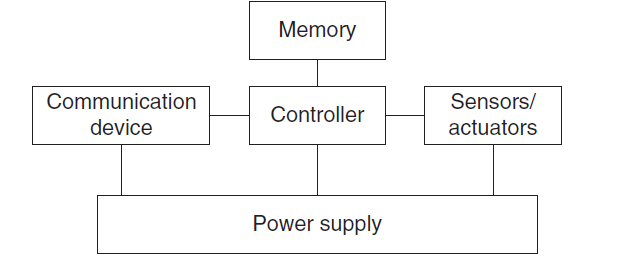
\includegraphics[width=10cm]{pictures/overview_node.png}
\caption{Visão Geral do Hardware de um Nó Sensor Sem Fio}
 \label{fig:overview}
\end{figure}

Nas próximas subseções serão apresentados, de forma resumida, alguns dos principais sensores existentes no mercado.

\subsubsection{Mica 2}
A plataforma \emph{Mica Mote} é comercializada pela \emph{Crossbow} e é uma das mais empregadas em projetos envolvendo RSSFs. A unidade de sensoriamento de cada nó \emph{Mica Mote} pode ser equipada com uma variedade de sensores, tais como acústico, temperatura, aceleração, luminosidade e pressão \cite{Ruiz2004}.

O \emph{Mica 2} é um nó sensor de baixo consumo de energia, podendo alcançar mais de um ano de autonomia utilizando pilhas AA. Este modelo possui um transceiver de rádio de 868/916 MHz multi-canal e utiliza \emph{Tiny OS} como sistema operacional.
O corpo deste sensor apresenta um conector de expansão de 51 pinos, isto permite que se conecte sensores de luz, temperatura, pressão, aceleração/sísmico, acústico, magnetismo, entre outros.

Devido suas características, o \emph{Mica 2} é indicado para aplicações como: segurança, vigilância, monitoramento de ambientes, redes de sensores de larga escala (mais de 1000 nós) e plataformas de computação distribuída.

Mais informações em: \cite{Mica2}.

\subsubsection{Mica Z}
O nó sensor \emph{Mica Z} é uma variação da plataforma \emph{Mica Mote}. Este nó possui diversas características comuns ao sensor \emph{Mica 2}, contudo, apresenta como suas maiores diferenças o uso de um rádio 2.4 GHz IEEE 802.15.4 e também sua capacidade de realizar transferências em taxas relativamente altas (250 kbps).

Este sensor pode ser utilizado em praticamente todos os tipos de aplicações do sensor \emph{Mica 2}. Em adição, este sensor é indicado para aplicações de medições acústica, de vídeo, vibração ou outras que demandem transmissões de alta taxa de transmissão, bem como aplicações de segurança e monitoramento \emph{indoor}.

Informações mais específicas podem ser encontradas em: \cite{MicaZ}.

\subsubsection{Iris}
Este modelo de nó sensor apresenta algumas características em comum com os nós da plataforma \emph{Mica Mote}, entretanto, apresenta avanços significativos em relação à plataforma anterior. Sua maior característica é o fato de possuir um rádio com alcance até três vezes maior que um sensor \emph{Mica Mote}, bem como o dobro de memória de programas.
Testes ao ar livre demonstraram que sensores utilizando esta plataforma foram capazes de se comunicar a uma distância de 500 metros.

Mais informações podem ser encontradas em: \cite{Iris}.

\subsubsection{TelosB}
\emph{TelosB} é uma plataforma \emph{Open Source} desenvolvida para permitir experimentação de ponta para a comunidade científica. Este sensor une diversas ferramentas essenciais para estudos de laboratório em um só sensor: Funcionalidade de programação via USB, um rádio IEE 802.15.4 com antena de integrada e uma CPU de baixo cosumo com memória extendida.
As características mais importantes deste nó sensor são a presença de interface USB para programação e uma memória flash externa de 1MB.

Informações mais detalhadas podem ser encontradas em: \cite{TelosB}.

\subsubsection{Imote 2}
O \emph{Imote 2} é uma plataforma avançada e de alto desempenho de nós sensores sem fio. Este modelo contém um processador Intel PXA271, com a capacidade de executar de baixas (16MHz) até frequências consideravelmente altas (416MHz).
Este tipo de sensor é indicado para aplicações que requeiram alto desempenho do nó sensor, como: processamento digital de imagens, monitoramento e análises industriais, monitoramento sísmico ou de vibração, etc.

Mais informações e características deste modelo podem ser visualizadas em: \cite{Imote}.


Na figura \ref{fig:nodes} podem ser visualizados os nós sensores citados nesta sessão.

\begin{figure}[h!]
\centering
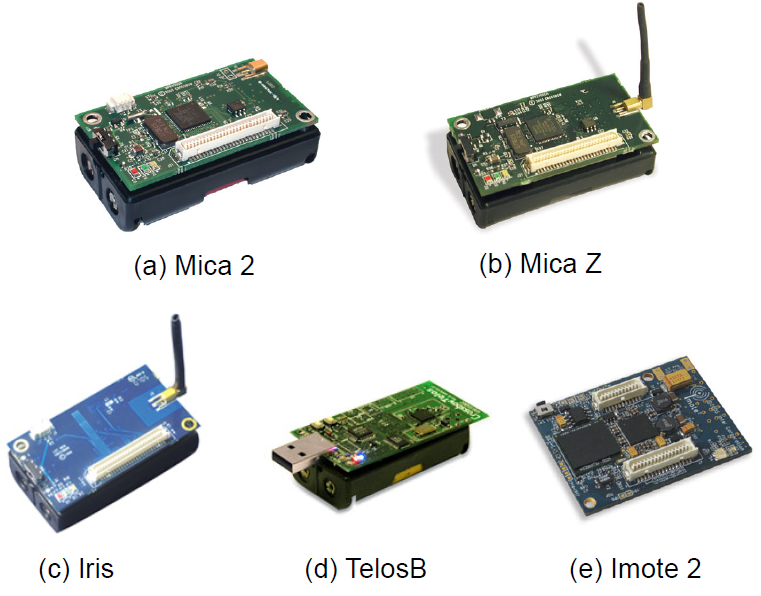
\includegraphics[width=12cm]{pictures/sensor_nodes.png}
\caption{Nós Sensores. (a) Mica 2, (b) Mica Z, (c) Iris, (d) TelosB, (e) Imote 2}
 \label{fig:nodes}
\end{figure}
\section{\uavs (\vants) }

\vants são definidos por \cite{uav_roadmap2005} como veículos aéreos que não carregam operadores humanos que são capazes de voar autonomamente ou serem pilotados remotamente e não são limitados por restrições humanas. Pelo fato de não carregarem pilotos, estes tipos de aeronaves podem ser sujeitos aos mais variados tipos de aplicação.
Exemplos básicos são áreas de baixo oxigênio, áreas contaminadas por resíduos tóxicos ou produtos químicos nocivos à saúde humana.

Estes veículos recentemente alcançaram um crescimento não previsto. Diversas aplicações em áreas civis e militares têm sido desenvolvidas nos mais diversos domínios \cite{Valavanis2007}.


Um forte fator de motivação no desenvolvimento de \vants é o fato dos mesmos ultrapassarem algumas barreiras onde as limitações humanas são fatores que restringem a execução de missões. Como exemplos, podem ser citados recuperação de desastres, áreas envenenadas ou com limitação de oxigênio, locais de difícil acesso onde necessitam-se de aeronaves de menor porte, entre outros casos \cite{uas_2009}. 

Atualmente existe uma grande diversidade de modelos de UAVs. Podendo variar em vários tamanhos, formatos, configurações e propósito.
Determinados \vants variam de aeronaves do tamanho de insetos à \vants com porte relativo a aviões comerciais \cite{Bone2003}.

Não se considerando apenas aspectos como segurança, mas também aspectos como extensão, \vants de vários tamanhos e modelos podem ser utilizados para monitoramento em recuperação de desastres, detecção de eventos, ente outros. 

Em aplicações militares, \vants trabalham por meio de execução de missões "3-D" ( \emph{Dull} - Tediosas, \emph{Dirty} - Sujas e \emph{Dangerous} - Perigosas) que não necessitam do uso de pilotos \cite{Bone2003}.


\cite{uav_roadmap2005} define missões 3-D como:
\begin{description}
\item[Tedioso: ]
\vants podem realizar missões consideradas tediosas para pilotos. Como exemplo a viagem rotineira de um vôo de 30 horas realizada por uma equipe do exército americano de Missouri até a Sérvia por 34 dias no conflito de Kosovo em 1999 \cite{uav_roadmap2005}. 

\item[Sujo: ]
Casos em que se torna necessário o monitoramento de alguma região contaminada. Entre 1946 e 1948, a força aérea (\emph{The Air Force}) e a marinha (\emph{The Navy}) americanos utilizaram \vants para recolherem amostras radioativas após detonação de bombas nucleares \cite{uav_roadmap2005}.

\item[Perigoso: ]
Missões de exploração ou reconhecimento podem apresentar riscos aos pilotos. Segundo \cite{uav_roadmap2005}, 25\%  dos pilotos dos grupos de reconhecimento do exército americano foram perdidos durante a Segunda Guerra Mundial no norte da África, enquanto somente 5\% dos pilotos de bombardeiros foram perdidos sobrevoando a Alemanha.

\end{description}

O restante desta sessão se preocupa em apresentar, de forma resumida, os avanços e pesquisa em \uavs. Na próxima subsessão serão apresentados os modelos básicos de \vants.

\subsection{Modelos e Arquiteturas de \vants}

Esta seção apresenta, de forma condensada, os avanços das pesquisas em modelos e arquiteturas de Veículos Aéreos Não Tripulados. Serão apresentados os principais modelos de \vants utilizados atualmente. Destaca-se o desenvolvimento de aeronaves direcionadas ao uso em aplicações militares.

Os principais modelos de \vants da atualidade foram projetados primeiramente com propósito de missões de reconhecimento e vigilância. Porém, esforços têm sido realizados para o desenvolvimento de \vants que representem maior representatividade em campos de batalha, como detectar alvos aéreos, monitorar movimento de tropas inimigas à auxílio de artilharia em batalhas \cite{Bone2003}.

A tabela ~\ref{tbl:categorization} apresenta as categorias de \vants reconhecidas pelos especialistas no assunto. Porém, por não ser objetivo deste trabalho realizar uma investigação detalhada a respeito dos modelos de \vants, será adotada a convenção proposta por \cite{Drew2005} para que o assunto não se extenda demasiadamente.
\begin{table}[h!]
\centering
\small
	\begin{tabular}{|p{3.0cm}| c c  c c c| }
		\hline
		Categoria&Alcance&Altitude&Autonomia&P.M.D.\footnotemark[1]&Atividade\\
		  	      & (km)         &   (km)     &(horas) & (kg)    & \\
		\hline
		\multicolumn{6} {| l |}{Táticos} \\
		\hline
		Nano& < 1 &100 &< 1 &< 0,025& sim \\
		Micro& < 10 &250 &1 &< 5 &sim \\
		Mini &< 10 &150 a 300& < 2& < 30& sim \\
		Close Range &10 a 30& 3.000& 2 a 4 &150& sim \\
		Short Range &30 a 70 &3.000 &3 a 6 &200 &sim \\
		Medium Range & 70 a 200 &5.000 &6 a 10 &1.250 &sim \\
		Medium Range Endurance  &> 500 &8.000 &10 a 18 &1.250& sim \\
		Low Altitude Deep Penetration &> 250 &50 a 9.000 &0,5 to 1 &350 &sim \\
		Low Altitude Long Endurance  &> 500 &3.000 &> 24 &< 30 &sim \\
		Medium Altitude Long Endurance &> 500 &14.000 &24 a 48 &1.500 &sim \\
		\hline

		\multicolumn{6} {| l |}{Estratégicos} \\
		\hline
		High Altitude Long Endurance & > 2000& 20.000 &24 a 48& 12.000& sim \\
		\hline
%
%		\multicolumn{6} {| l |}{Propósito Especial} \\
%		\hline
%		Unmanned Combat Aerial Vehicle & approx. 1500&10.000& approx. 2& 10.000& sim \\
%		Lethal & 300 & 4.000& 3 a 4 &250& sim \\
%		Decoy  &0 a 500 &5.000 &< 4 &250 &sim \\
%		Stratospheric & > 2000 &20.000 a 30.000 &> 48 &TBD\footnote{\emph{To Be Defined} - A Definir} &não \\
%		Exo-stratospheric & TBD &> 30.000 &TBD& TBD& não\\
%		Space  &TBD &TBD &TBD& TBD& não\\
%		\hline
	\end{tabular}
	
	\caption{Categorias de \vants. Fonte: 2009/2010 UAS Yearbook - UAS: The Global Perspective - 7th Edition}
	\label{tbl:categorization}
\end{table}



\cite{Drew2005} dividem os \vants em duas principais classes baseadas na extensão das aeronaves. Neste trabalho serão consideradas como Grande Porte e Pequeno Porte (Micro, Portáteis e Multi-missões).

O foco deste trabalho não é uma investigação sobre os modelos e arquiteturas de \vants. Portanto,  neste tópico serão apresentados, de forma resumida, alguns modelos comuns de UAVs. Mais informações sobre arquiteturas de \vants podem ser encontradas em \cite{Drew2005,uav_roadmap2005, Bone2003,Holder2001}.

\footnotetext[1]{Peso Máximo de Decolagem - É o peso máximo permitido para que um avião consiga realizar vôos em plena capacidade. }
\addtocounter{footnote}{1}

\subsubsection{\vants de Grande Porte}
Segundo \cite{Drew2005}, \vants de grande porte têm sistemas de lançamento e recuperação que podem ser separados dos seus sistemas de controle e exploração de dados. Ou seja, apresentam mecanismos que podem ser controlados separadamente, como por exemplo, coleta das informações e comunicação via satélite.



 \paragraph{\emph{Global Hawk} }

 É o \vant mais caro já produzido. Este \vant é capaz de alcançar altitudes elevadas (65.000 pés\footnote{A medida de 1 pé é de aproximadamente 30cm.}), e longos períodos de ativididade de 28 a 32 horas. Este modelo é capaz de prover imagens próximas a tempo real em grandes áreas geográficas (cerca de 40.000 nm$^{2}$ \footnote{Milhas náuticas quadradas. 1 milha náutica representa 1,828 km.} por dia) \cite{uav_roadmap2005}.

Segundo \cite{Drew2005}, o \emph{Global Hawk} foi o primeiro \vant a realizar uma viagem trans-pacífico, quando voou da Califórnia à Austrália em 22-23 de Abril de 2001.

O preço de um \emph{Global Hawk} completo é próximo de 54 milhões de dólares. E o preço de cada estação terrestre para controle
é de 16 milhões.

\begin{figure}[h!]
\centering
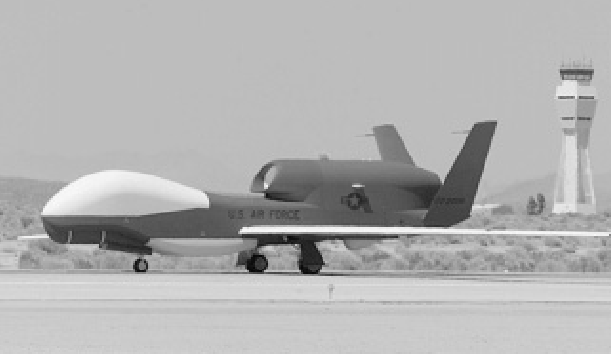
\includegraphics[width=10cm]{pictures/global_hawk.png}
\caption{Global Hawk}
 \label{fig:global_hawk}
\end{figure}


Este modelo apresenta 13,5 metros de extensão, peso de 12.144 quilos e possui o tamanho comparável ao de um jato comercial de médio porte. 



Mais informações podem ser encontradas em:  \cite{Drew2005,uav_roadmap2005,Bone2003}.


\paragraph{ \emph{Predator} }

 O modelo \emph{Predator} é um \vant  de grande porte, considerado de média a alta altitude (15.000 a 25.000 pés), apresenta 
uma extensão de aproximadamente 11 metros,  4.767 quilos de peso e autonomia de vôo de 16 a 30 horas.

\begin{figure}[h!]
\centering
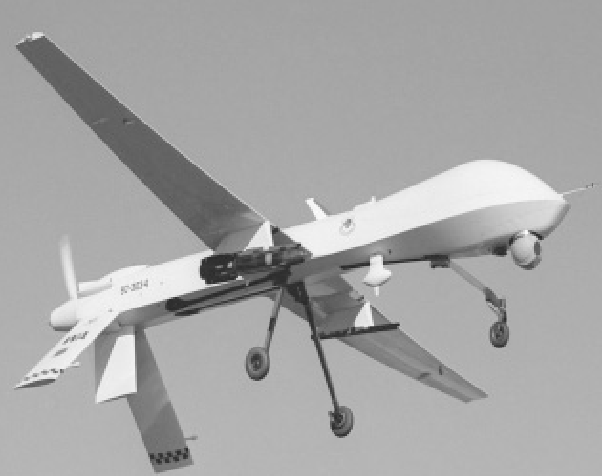
\includegraphics[width=10cm]{pictures/predator.png}
\caption{Predator}
 \label{fig:predator}
\end{figure}

A primeiro propósito deste modelo de \vant é atuar como vigilante em uma determinada área de interesse. Este \vant é equipado com uma variedade de sensores para capturar imagens de alta resolução em determinadas áreas.
O segundo propósito para o desenvolvimento deste modelo de aeronave é atuar em conjunto de inteligente de \uavs. 

Cada \emph{Predator} tem um custo aproximado de 4.5 milhões de dólares. Um sistema completo de \emph{Predator}s custa em média 30 milhões de dólares.

Para mais informações sobre este modelo:  \cite{Drew2005,uav_roadmap2005,Bone2003}.



\subsubsection{\vants de Pequeno Porte}

Em \cite{Drew2005}, \vants de Pequeno Porte são divididos nas seguintes subclasses:

\begin{description}

\item[Micro-\vants: ]
São aeronaves de menor porte e geralmente são utilizadas para missões de reconhecimento, pois seu tamanho reduzido permite uma grande versatilidade. Uma característica importante é que estes modelos são indicados somente para operações durante o dia e com boas condições climáticas, visto que as restrições de tamanho dificultam a locomoção em más condições climáticas. Estes modelos são projetados para carregarem cargas de peso inferior a 200g.

\item[Portáteis: ]
São modelos direcionados à aplicações de pequenos times de \vants. Estes modelos se adaptam bem à aplicações colaborativas. Podem ser carregados e lançados por uma pessoa. Geralmente estes \vants apresentam autonomia de vôo de aproximadamente 1 a 2 horas, e normalmente carregam cargas de até 25 kg.

\item[Multi-Missão: ]
Conhecidos como \vants  de propósito geral, estes são os maiores entre os menores modelos de \vants e geralmente apresentam autonomia de voo de 10 a 12 horas e possuem capacidade para carregar cargas de 25 a 110 kg. Estes \vants são projetados para missões operacionais variadas, sendo considerados as aeronaves mais versáteis da categoria. Exemplos comuns de aplicações são: carregamento de suprimentos para o campo de batalha, distribuição (\emph{deployment}) de sensores em uma região, monitoramento, entre outros.

\end{description}


\paragraph{\emph{RAVEN}}
É um \vant portátil que carrega câmeras infra-vermelho frontais e laterais. Este modelo pode ser pilotado remotamente ou através de vôo autônomo baseado em GPS. Em muitos casos 
este modelo é utilizado para missões de reconhecimento e vigilância, destacando-se no uso para reconhecimento noturno devido o uso de suas câmeras infra-vermelhas.

Este modelo pode sobrevoar altitudes de no máximo 14.000 pés, porém seus usos mais comuns são em missões variando de 150 a 500 pés de altura. Possui um raio de alcance de 
13 a 18,5 km e autonomia de 60 a 90 minutos, alcançando velocidade máxima de 110 km/h e velocidade de cruzeiro de aproximadamente 50 km/h \cite{uas_2009}. 

A instalação de um sistema composto por dois \emph{RAVENs} custa aproximadamente 139.000 dólares \cite{Drew2005}. 

Nas figuras ~\ref{fig:raven} e  pode ser vista a operação de lançamento de um \vant do tipo \emph{RAVEN}.

\begin{figure}[h!]
\centering
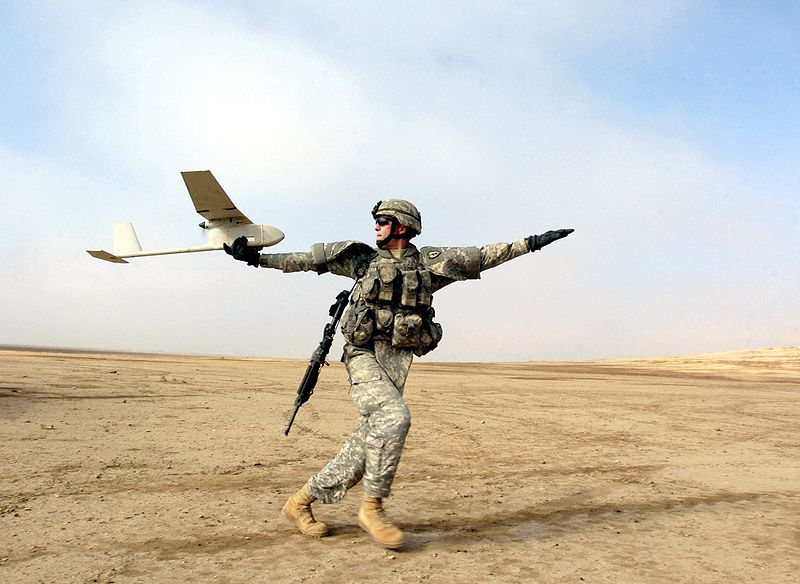
\includegraphics[width=10cm]{pictures/launching_raven.jpg}
\caption{Soldado americano lançando um \emph{RAVEN} }
 \label{fig:raven}
\end{figure}




\paragraph{ \emph{Pointer}}
Este \vant  portátil foi desenvolvido para prover dados em tempo real em uma grande variedade de aplicações. Sua missão primária é a de reconhecimento e vigilância de áreas
utilizando sensores EO\footnote{Sensor Eletro-Óptico.} e IR\footnote{Infra-red, em português: Infra-Vermelho.}, bem como sensores de detecção química. Este modelo apresenta comprimento de asa de 9 pés e pesa apenas 3,7 kg. Um \emph{Pointer} tem autonomia de vôo de aproximadamente 2 horas e pode alcançar altitudes de até 500 pés carregando cargas de no máximo 500g \cite{uas_2009}. Um sistema de dois \emph{Pointers} custa aproximadamente 133.000 dólares \cite{Bone2003}. 

Na figura ~\ref{fig:launching_pointer} pode ser visto o lançamento de um \emph{Pointer}. 

\begin{figure}[h!]
\centering
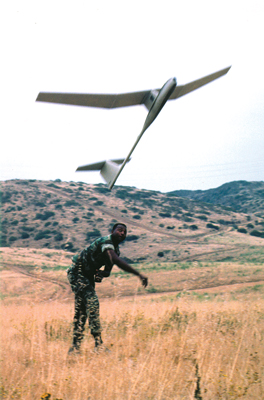
\includegraphics[width=6cm]{pictures/launching_pointer.jpg}
\caption{Lançamento de um \emph{Pointer} }
 \label{fig:launching_pointer}
\end{figure}


\paragraph{ \emph{BATCAM}}
O \emph{The Battlefield Air Targeting Camera Micro Air
Vehicle} (BATCAM) é um modelo altamente avançado de Micro-\vant. Este \vant  é menor que outros modelos como \emph{Pointer}, \emph{Raven} e \emph{FPASS}.
O \emph{BATCAM} tem um peso de aproximadamente700g, apresenta uma autonomia de vôo de apenas 30 minutos, altitude de vôo de 500 pés e uma capacidade de carga de
apenas 200g. Este modelo foi construído para missões de reconhecimento e carrega sensores IR e EO.

Devido o seu tamanho reduzido. Este modelo pode ser utilizado em diversos tipos de operação, como infiltração, monitoramento e vigilância \cite{Drew2005}. 


Na figura ~\ref{fig:holding_batcam} é apresentado um sistema \emph{BATCAM}.

\begin{figure}[h!]
\centering
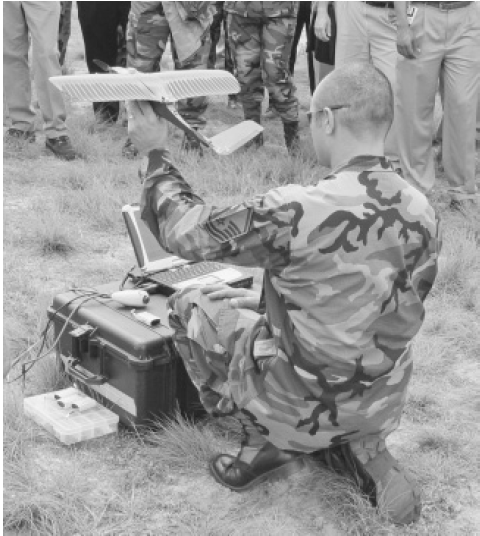
\includegraphics[width=10cm]{pictures/batcam_system.png}
\caption{ Soldado operando um \emph{BATCAM} }
 \label{fig:holding_batcam}
\end{figure}


\paragraph{ \emph{Dragon Eye}}
O \vant \emph{Dragon Eye} foi projetado para missões de reconhecimento, vigilância e detecção de alvos. Com um comprimento de asa de apenas 18 cm e peso de 2,5 kg, este modelo pode ser carregado ate mesmo em uma mochila e ser lançado facilmente em diversos tipos de situação.

Este modelo pode voar em velocidades de aproximadamente 75 km/h, cobrindo uma área de até 10km e retornando em 1 hora. Geralmente alcança altitudes de 300 a 500 pés.
Devido a sua grande versatilidade, este \vant tem sido utilizado em diversas aplicações urbanas \cite{Drew2005,uav_roadmap2005}.

Um sistema \emph{Dragon Eye} é composto por 2 veículos aéreos, 4 câmeras, 2 frentes removíveis e uma estação terrestre de controle. O custo de um sistema \emph{Dragon Eye} é
de aproximadamente 65.000 dólares. Na figura ~\ref{fig:dragon_eye} pode ser visto um sistema \emph{Dragon Eye}.


\begin{figure}[h!]
\centering
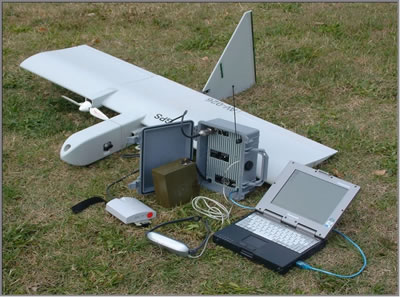
\includegraphics[width=10cm]{pictures/dragon_eye_system.jpg}
\caption{Sistema \emph{Dragon Eye} }
 \label{fig:dragon_eye}
\end{figure}




\subsection{Aplicações utilizando \vants}
Atualmente, a pesquisa em \vants tem se concentrado fortamente em aplicações militares, variando de aplicações de monitoramento, vigilância, suporte de ataque aéreo, entre outros. Atualmente, segundo \cite{Valavanis2007} a pesquisa em diferentes tipos de aplicação (não somente militares) tem crescido e ampliado os horizontes de desenvolvimento.

Na tabela~\ref{tbl:vants_por_ano} é possível visualizar o desenvolvimento das aplicações utilizando \vants nos últimos anos.


\begin{table}[h!]
\centering
	\begin{tabular}{| l | c | c | c | c | c | c |}
		\hline
		Aplicações/Ano & 2004 & 2005 & 2006 & 2007 & 2008 & 2009 \\
		\cline{2-7}
		 & Qt & Qt & Qt & Qt & Qt & Qt  \\
		\hline
		Civil/Comercial  & 33 &  55  & 47  & 61  & 115  & 150 \\
		%\hline
		Militar  & 362  & 397  & 413  & 491  & 578  & 683 \\
		%\hline
		Propósito Geral &  39  & 44  & 77  & 117  & 242  & 260 \\
		%\hline
		Pesquisa  & 43  & 35  & 31  & 46  & 54  & 66 \\
		%\hline
		Desenvolvimento de \vants &   & 219  & 217  & 269  & 293  & 329 \\
		\hline
	\end{tabular}

	\caption{Aplicações de \vants por ano. Fonte: 2009/2010 UAS Yearbook - UAS: The Global Perspective - 7th Edition}
	\label{tbl:vants_por_ano}
\end{table}

Na figura~\ref{fig:qt_uav_app} podem ser visualizadas as quantidades de \vants utilizadas nos diferentes tipos de aplicações.

\begin{figure}[h!]
\centering
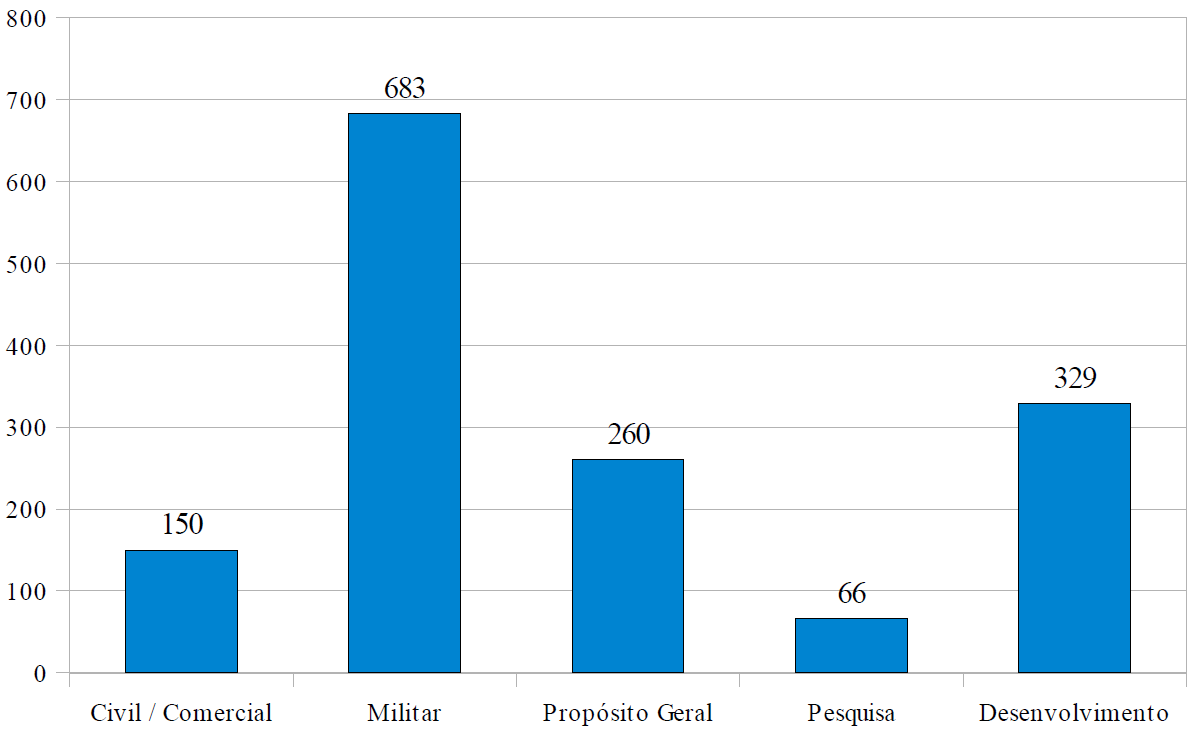
\includegraphics[width=13cm]{pictures/qt_uavs_app.png}
\caption{Quantidade de \vants por classe de aplicação. Fonte: 2009/2010 UAS Yearbook - UAS: The Global Perspective - 7th Edition}
 \label{fig:qt_uav_app}
\end{figure}

Pode-se notar um aumento significativo no número de aplicações comerciais e de propósito geral nos anos de 2008 e 2009.

\subsection{Desenvolvimento de \vants}

Diversas nações têm se destacado quanto ao desenvolvimento de \vants. Os Estados Unidos é o país que atualmente possui mais aeronaves produzidas (386), e representa 32,44\% da
produção mundial de aeronaves não tripuladas. Outras nações como Israel (83 - 6,97\%),  França (77 unidades - 6,47\%), Rússia (59 unidades - 4,96\%) e Reino Unido (65 - 5,46\%) também têm apresentado resultados significativos quanto ao número de \vants produzidos. O Brasil, ainda iniciando suas pesquisa em \vants, possui 6 unidades produzidas, contabilizando apenas 0,5\% das aeronaves não tripuladas produzidas no mundo.

Na tabela~\ref{tbl:country} encontram-se os dados resumidos do desenvolvimento de \vants em âmbito mundial. Informações mais detalhadas encontram-se em anexo.

\begin{table}[h!]
\centering
	\begin{tabular}{| l | c | c |}
		\hline
		País & Número de Aeronaves & \% \\
		\hline
		EUA & 386 & 32,44 \\
		Israel & 83 & 6,97 \\
		França & 77 & 6,47 \\
		Reino Unido & 65 & 5,46 \\
		Iran & 38 & 3,19 \\
		Brasil & 6 & 0,50\\
		Outros Países & 535 & 44,97 \\
		\hline
	\end{tabular}

	\caption{Desenvolvimento de \vants por nação. Fonte: 2009/2010 UAS Yearbook - UAS: The Global Perspective - 7th Edition}
	\label{tbl:country}
\end{table}


\subsection{Pesquisas em \vants}
Diversos esforços têm sido realizados nas pesquisas sobre \uavs, bem como diversas aplicações têm sido desenvolvidas. Este tópico demonstrará alguns avanços da pesquisa e
utilização prática de \vants em diversos cenários.

\begin{description}

\item[Exploração em Regiões Polares: ]
\cite{Storvold2009} mostra em \emph{Scientific UAS Missions in the Polar Regions} alguns avanços do uso de \vants em aplicações de exploração e monitoramento de regiões polares. A utilização de aeronaves não tripuladas neste tipo de missão se justifica pelo fato das limitações de resoluções espaciais e temporais dos satélites que cobrem estas áreas. O uso de \vants proporciona medidas mais precisas pelo fato de serem realizadas com mais proximidade. Outro fator destacado na utilização de \vants para este tipo de exploração é que a utilização de
aeronaves pilotadas por humanos neste tipo de região se apresenta altamente custoso e perigoso devido as condições climáticas desfavoráveis da região. A utilização de \vants proporcionou redução dos gastos e melhorou a acurácia das medidas na região. 

\item[Recuperação de Desastres e Incêndios: ]
Uma grande variedade de organizações (além das organizações militares), ultimamente, tem considerado o uso de \vants  numa grande variedade de aplicações. O grupo de bombeiros
WMFS (\emph{West Midlands Fire Service}), do Reino Unido, tem utilizado o sistema \emph{ISiS} para a suporte em casos de desastres. \cite{Mika2009} relata casos de uso do sistema \emph{ISiS} para suporte em diversos desastres. A utilização de câmeras de alta resolução instaladas em \vants de pequeno porte permite que os bombeiros visualizem a situação e provê suporte para que sejam tomadas decisões mais coerentes com cada caso.

\begin{figure}[h!]
\centering
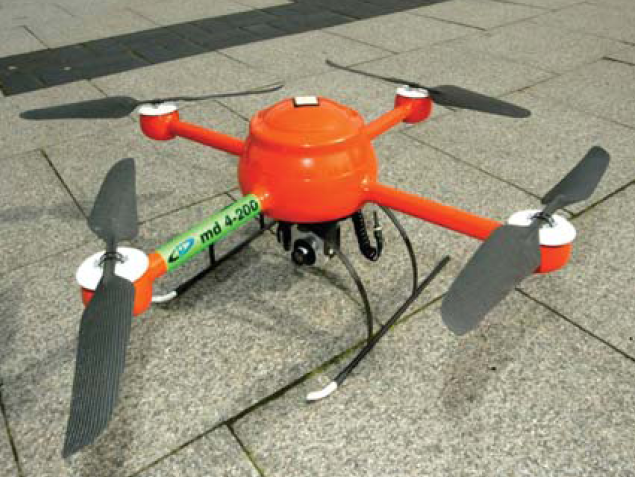
\includegraphics[width=10cm]{pictures/mq4200.png}
\caption{ \emph{MD4-200}: \vant utilizado por \emph{West Midlands Fire Service} para reconhecimento em locais de desastre. }
 \label{fig:md4-200}
\end{figure}

O \vant utilizado nas missões do WMFS é conhecido como MD4-200. Este \vant é composto predominantente de fibra de carbono e plástico reforçado. Tem um peso de 900g e apresenta três principais sensores: Câmera de vídeo de alta resolução, câmera fotográfica de alta resolução (12 mega pixels) e um sensor infra-vermelho. Este modelo também possui alcance de 3km a partir da estação base. Na figura~\ref{fig:md4-200} pode ser visualizado um MD4-200 utilizado nas operações citadas.

Por volta de 20\% dos terremotos de larga escala ocorrem no Japão, e também 7\% dos vulcões em atividade estão localizados neste país. Danos por tempestades, inundações e nevascas também têm sido comuns neste território. \cite{Sasa2008} demonstram os avanços nas pesquisas do \emph{JAXA Aviation Program Group} e propõem soluções para a melhoria da infraestrutura de previsão de desastres japonesa.

\item[Controle Autônomo: ]
Em \cite{Semsch2009} são tratados problemas de controle autônomo de \vants. Neste trabalho os autores apresentam problemas em que se necessita controlar um time de vários \vants para que se promova vigilância em ambientes urbanos complexos. São demonstrados problemas complexos como monitorar áreas de difícil visualização, como regiões com prédios altos e ruas estreitas. Outros autores como \cite{KimAndKim} e \cite{Sarmiento2004} também trabalharam problemas de controle autônomo e oclusão.

\item[ Sistemas para evitar colisão (\emph{Collision Avoidance}):]
Diversos esforços têm sido gastos no desenvolvimento de sistemas para se evitar colisão em grupos de \vants (\emph{Collsion Avoidance}). Tratam-se de casos onde se torna necessário controlar grupos de \vants (ou apenas um único) para que os mesmos não colidam entre si, ou colidam com algum obstáculo.

Segundo \cite{Hutchings2007}, sistemas de \emph{Collision Avoidance} ou \emph{Sensing Avoidance} são divididos em:
	\begin{description}
		\item[S\&A estratégico: ]  Conflitos potenciais são detectados a longo prazo. Isto permite que a rota seja reprogramada e o objeto de conflito possa ser evitado.
		\item[Avisos de Resolução de Conflitos: ] Algum agente externo envia um aviso para que o \vant altere sua rota. O \vant deve esperar e aceitar avisos constantemente.
		\item[Controle Autônomo de S\&A: ] O \vant realiza uma manobra num tempo mínimo de segurança para se evitar a colisão.
	\end{description}

Trabalhos relacionados podem ser encontrados em \cite{Hutchings2007,Bryner2007,Deschenes2004,Taylor2005}, entre outros.

\end{description}

Nesta seção foram apresentados brevemente a motivação, os tipos e modelos de \vants, bem como algumas informações a respeito do desenvolvimento, pesquisas e investimentos nesta área. Muitos outros trabalhos e aplicações de \vants podem ser encontrados e demonstrados. Porém, não é foco deste trabalho fazer um levantamento completo do estado da arte de \uavs. 

\section{Pesquisas em RSSFs e UAVs}

Redes de sensores sem fio com nós estáticos (sem movimento) têm sido desenvolvidas, testadas e aplicadas em diversas atividades de detecção e monitoramento de fenômenos.
Contudo, \rssfs estáticas apresentam algumas limitações. O uso de nós sensores móveis pode prover melhorias significativas. Nós moveis podem prover meios de se observar estes fenômenos
com uma maior riquesa de detalhes e granularidade. Ainda mais, nós sensores móveis podem colher informações dos nós sensores estáticos no momento em que transitam
 pela região de interesse \cite{Aware}. 

Aliado às preocupações apresentados, um novo desafio em \rssfs é a coordenação de nós sensores heterogêneos com diferentes capacidades de sensoriamento, mobilidade e computação em uma única rede \cite{Freitas2009}. 

Em complemento, as capacidades e papéis dos Veículos Aéreos Não Tripulados têm evoluido e têm requerido novos conceitos e técnicas para suas operações. Por exemplo, \vants atuais tipicamente requerem vários operadores, mas os próximos \vants serão projetados para tomar decisões táticas autonomamente e serão integrados em times que se coordenam para alcançar objetivos de mais alto nível \cite{Richards2002, Mehdi2003}. 

Neste contexto existe uma proposta para se unir estes três desafios e preocupações (nós sensores móveis, coordenação de nós sensores heterogêneos e controle autônomo de UAVs): a utilização de \uavs em colaboração com redes de sensores sem fio. Este novo modelo de cooperação engloba os requisitos anteriormente citados. A idéia é que \vants sejam equipados com uma variedade de sensores e uma interface de comunicação sem fio, e a partir disso se estabeleçam conexões \emph{wireless} entre as aeronaves e os nós sensores estáticos da rede. 

Esta área de pesquisa encontra-se ainda em expansão, consequentemente pouca literatura consolidade encontra-se disponível. Os principais esforços encontram-se na utilização dos nós sensores para realizar o controle do \vant, ou o inverso, utilização de \vants para coordenação da RSSF.


Alguns dos primeiros passos neste tipo de combinação surgiram com o projeto \emph{Aware - Platform for Autonomous Self-Deploying and Operation of Wireless Sensor-
Actuator Networks Cooperating with AeRial ObjEcts}. O principal objetivo do sistema \emph{Aware} é a detecção de eventos por meio de sensores terrestres, e posteriormente a entrega do alarme a um UAV. Outro objetivo do \emph{Aware} é a reparação automática de rede. Em casos onde nós são danificados ou perdidos, helicópteros não tripulados deverão ser capazes de reparar a conectividade da rede. Detalhes sobre a plataforma \emph{Aware} podem ser encontrados em \cite{Aware, Aware2}


\cite{Lucchi2007} consideram a utilização de \vants como \emph{sinks}(nós concentradores) móveis em uma \rssf. Neste trabalho, \vants são utilizados para coletar os dados medidos pela rede de sensores e realizar tarefas de fusão de dados. Além disso, são apresentos critérios e técnicas para tratamento de ruído e falhas ocorridas na comunicação entre os nós sensores e os \vants utilizados.

\vants também podem ser utilizados para prover suporte a algoritmos de localização em \rssfs. \cite{Guerrero2009} propoem uma solução baseada em agentes móveis para se definir a localização geográfica de cada nó sensor da rede. É utilizado um \vant carregando uma antena direcional e um dispositivo GPS. Basicamente, concentra-se na medida da intensidade do sinal recebida de cada nó, e a partir desta intensidade torna-se possível calcular a distância entre o \vant e o nó sensor em questão.

\cite{Freitas20092} apresentam uma avaliação sobre estratégias de coordenação de nós sensores heterogêneos (\rssf e UAVs). Uma destas avaliações é um estudo baseado em ferormônios digitais para realizar uma comunicação mais eficiente entre os nós sensores estáticos e os UAVs. A segunda avalição é a definição de heurísticas, para casos em que se encontram vários \vants em uma mesma missão, para se selecionar o \vant mais hábil a tratar os alarmes acionados pela RSSF.




\newpage\section{Metodologia}
\label{chap:Metodologia}


O trabalho, quanto à sua natureza, é considerado como de Pesquisa Aplicada, pois visa o tratamento de um problema concreto. Espera-se ao fim, que a própria pesquisa apresente resultados sólidos em se tratando da resolução do problema apresentado.

Quanto aos objetivos, se classifica como pesquisa exploratória, visto o objetivo de combinar práticas existentes (algoritmos auto-organizáveis) em busca da resolução de um problema.

No que se refere aos procedimentos, é considerada como pesquisa experimental, novamente por se apresentar como aplicação de métodos e técnicas. Para a realização do trabalho, se fará uso de ensaios e estudos de laboratório. Onde, a partir do simulador GRUBiX, poderão ser feitas as simulações, testes e avaliações dos algoritmos.
              
Ainda em relação às práticas metodológicas, a pesquisa também se classifica como quantitativa. Serão realizados testes, simulações e avaliações de forma quantitativa. Ao fim serão comparados os valores numéricos de cada experimento.

\subsection{Procedimentos Metodológicos}

Os experimentos realizados neste trabalho basearam-se em simulação. O uso de simulação justificou-se pela complexidade em se aplicar o algoritmo proposto em uma grande quantidade de nós sensores, seja em questões financeiras ou de tempo para se testar o algoritmo em uma grande variedade de cenários.

A próxima seção introduz os conceitos referentes ao simulador utilizado, bem como os conceitos de Simulação Orientada a Eventos.

\subsubsection{\emph{GRUBiX} e Simulação Orientada a Eventos}
Para desenvolvimento do algoritmo proposto neste trabalho, foi utilizado o simulador de redes sem fio \emph{GRUBiX}, desenvolvido no Departamento de Ciência da Computação, pelo grupo de pesquisas GRUBi, da Universidade Federal de Lavras.

Este simulador é uma evolução do projeto \emph{Shox}\cite{shox}. Assim como o \emph{Shox}, o simulador \emph{GRUBiX} caracteriza-se como um ambiente de simulação orientado a eventos. De forma simplificada, em um ambiente de simulação orientado a eventos, a linha do tempo de uma simulação é representada por uma lista de eventos, onde cada novo evento é inserido nesta lista. A posição em que cada evento é inserido nesta lista varia de acordo com o momento em que cada evento deve ocorrer.

Adicionalmente, estes simuladores disponibilizam uma API\footnote{\emph{Application Programming Interface}} para que se possa desenvolver toda a pilha de protocolos presente em um nó sensor sem fio. Esta disponibilidade permite que cada camada da pilha de protocolos seja personalizada de acordo com as necessidades de cada aplicação.

Assim como o \emph{Shox}, o simulador \emph{GRUBiX} utiliza a linguagem de programação Java. O uso de uma linguagem orientada a objetos, neste caso Java, indica que as camadas da pilha de protocolos sejam modeladas como objetos. O uso desta modelagem orientada a objetos permite que cada camada seja personalizada através de mecanismos de herança. Portanto, basta que a nova camada personalizada herde as funcionalidades de uma camada base para que se tenha a possibilidade de alterar o comportamento padrão da camada.

\subsubsection{Métodos}
Compreendidos os conceitos apresentados na sessão anterior, o desenvolvimento deste trabalho caracteriza-se por um algoritmo desenvolvido sobre a camada de aplicação da pilha de protocolos dos nós sensores sem fio e dos \vants.

Como discutido anteriormente, o \emph{GRUBiX} é escrito na linguagem de programação Java, e utiliza-se de conceitos de herança para o desenvolvimento das simulações. Portanto, o código das simulações deste trabalho foram todos escritos nesta linguagem de programação. Os próximos capítulos discutem o funcionamento do algoritmo e os resultados apresentados.





\newpage\section{Desenvolvimento}
\label{chap:Desenvolvimento}

Este capítulo discute o funcionamento do algoritmo desenvolvido para a coordenação da \rssf em conjunto com 
\vants. As próximas seções descrevem o problema tratado e apresenta a solução para a resolução deste problema.


\subsection{Descrição do Problema}

Este trabalho preocupa-se em pesquisar e desenvolver uma estratégia para a
coordenação de uma rede de sensores heterogênea. A rede em questão deve ser
utilizada para prover tarefas de monitoramento e vigilância de um ambiente de
interesse. Como ferramentas para se realizar estas tarefas de monitoramento são
utilizados nós sensores terrestres equipados com diversas interfaces de
sensoriamento e \vants também equipados com interfaces de sensoriamento e
enlaces de comunicação sem fio.

A justificativa e motivação para a utilização destes diferentes tipos de nós
sensores encontra-se no fato de que um nó sensor terrestre usual apresenta
capacidade computacional reduzida. Portanto, estes tipos de nós são incapazes de
cumprir todas as tarefas da rede individualmente. Em contrapartida, estes nós
sensores convencionais geralmente possuem custos reduzidos, o que propicia o uso
de vários sensores para a realização de missões. 

\uavs podem variar em tamanhos, formas, configurações e propósitos, adequando-se
a diversos cenários de aplicação. Neste trabalho, justifica-se o uso de
\emph{Mini-UAVs} (UAVs Multi-Missão), que são aeronaves de custo não tão elevado
quando comparados aos custos de aeronaves de grande porte. Portanto, uma
alternativa interessante é a utilização de \emph{Mini-UAVs} carregando uma
variedade de sensores específicos (sensores como câmeras de alta resolução,
infra-vermelho, GPS, etc) e que possuam poder computacional superior aos nós
sensores terrestres, permitindo assim que os \vants possam realizar missões e
medidas mais sensíveis e específicas.

Esta relação entre sensores terrestres simples e de baixo custo e \vants
relativamente mais caros justifica o uso de vários sensores simples espalhados
pela área de interesse em conjunto com alguns poucos, ou apenas um, \vant para
realizar as tarefas mais específicas. 

Por fim, o problema tratado é o desenvolvimento de uma estratégia eficientes para detecção de um evento através dos
nós sensores mais simples e garantir que as mensagens sejam entregues aos \vants
mais hábeis a tratar o evento de forma específica.

Dentre uma infinidade de exemplos de monitoramento de áreas de interesse,
podem ser citados:

\begin{description}
 \item [Áreas Militares de Acesso Restrito:] Locais de acesso proibido, onde se deseja detectar a presença de intrusos.
 \item [Detecção de Fenômenos Físicos:] São áreas onde se pretende detectar a ocorrência de fenômenos como alteração de
temperatura, umidade, sons, etc.
 \item [Observação de Animais:] Aplicações em que o objetivo seja o monitoramento de espécies de animais, como, por exemplo,
a presença de uma espécie incomum em uma determinada área.
\end{description}



Observados os problemas e exemplos expostos anteriormente, este trabalho apresenta algumas soluções para se aprimorar
a utilização de veículos aéreos não tripulados em conjunto com redes de sensores sem fio.

Resumidamente, os algoritmos desenvolvidos são:

\begin{description}

	\item[ (a) Distribuição de Ferormônio: ] o \vant sobrevoa continuamente
a área de interesse da aplicação. Enquanto sobrevoa esta área, o \vant deve se
comunicar com os nós sensores que se encontram abaixo do mesmo, estes nós
armazenam um valor com a intensidade do sinal com que a mensagem foi recebida.
Neste momento é formado um gradiente que corresponde a um rastro artificial da aeronave.

	\item[ (b) Detecção e Propagação do Evento:] quando um evento é
detectado, os nós sensores terrestres devem realizar uma negociação a fim de
enviar uma mensagem de alarme para os \vants presentes na área. Esta mensagem
deve encontrar o rastro de ferormônio formado em (a) e prosseguir até o \vant
mais hábil para tratar o evento ocorrido.

%	\item[ (c) Reforço de Conectividade da Rede:] algoritmo utilizado para reforçar a conectividade da rede em casos de falhas em algum nó.

%% Este aqui vai par os trabalhos futuros

% 	\item[ (c) \emph{Tracking} e Perseguição do Intruso: ] no momento em que
% os nós sensores detectam a presença de um dado evento, como exemplo o caso de um
% intruso, providências devem ser tomadas para que o mesmo alarme de evento não
% seja repetido. Por exemplo, o nó sensor X percebe a presença de um intruso na
% área, poucos segundos depois o nó Y também percebe o mesmo intruso, se ambos os
% nós enviarem um alarme aos \vants pode ocorrer carga excessiva na rede, bem como
% gerar confusão entre os \vants, pois os mesmos são interrompidos e reprogramados
% a cada alarme recebido. Portanto, na ocorrência de um evento, os nós da micro
% região onde onde houve a detecção devem alterar seu modo de trabalho, realizando
% assim uma perseguição e rastreamento, marcando uma trilha de mobilidade do
% evento, ao invés de soar os alarmes novamente.

%\item[ (b) Reforço dos Rastros de Ferormônio:] Em situações em que se utiliza mais de uma aeronave pode se 
%tornar interessante desenvolver uma política de reforço dos rastros de ferormônio construídos em (a) por cada \vant.
%Nesse caso, cada \vant pode reforçar o gradiente de todos os outros, desde que seus rastros se encontrem em algum ponto
%da área de interesse.

\end{description}

As próximas seções discutem o problema apresentado em diferentes perspectivas, apresentando suas peculiaridades e possíveis
soluções. Os algoritmos são introduzidos em uma sequência lógica para que se torne possível o entendimento do problema em questão. Vale 
ressaltar que esta ordem foi escolhida para um melhor entendimento do problema, visto que cada seção apresenta dependência em relação aos conceitos
apresentados nas seções anteriores. 

\subsection{Detecção de Eventos}
Para que um sistema de monitoramento realize seu papel de forma eficaz, espera-se, no mínimo, que este seja capaz de detectar eventos. Todo o funcionamento
de um sistema deste tipo depende da detecção dos eventos de interesse. Contudo, o foco deste trabalho não está no desenvolvimento de algoritmos para 
detecção de eventos. Portanto, adotou-se uma abordagem básica para a detecção de eventos pela \rssf, visto que a preocupação principal deste trabalho não se concentra neste problema.

A estratégia de detecção dos eventos de interesse escolhida pode ser considerada simples. Entretanto, apresenta-se eficaz para o desenvolvimento deste trabalho.
Cada nó sensor dá rede possui sensores dos mais variados tipos: umidade, temperatura, pressão, eletro-magnético, etc. Cada um destes sensores pode ser
configurado de modo que possua um limite\footnote{O termo limite pode ser encontrado em literaturas internacionais como \emph{threshold}} aceitável de medição em determinado parâmetro. Definidos os limites, são agendadas algumas medições para aquele sensor. Em caso de uma medição exceder o limite aceitável
para aquele parâmetro o nó sensor pode considerar este fenômeno como um evento de interesse detectado. Se a medição não exceder o limite, o nó simplesmente
deverá agendar outra leitura em tempo futuro.

O algoritmo a seguir demonstra o algoritmo em formato simplificado. \\

\begin{algorithm}[H]
%	\SetAlgoLined
	
	\SetKwFunction{realizarMedicaoNoAmbiente}{realizarMedicaoNoAmbiente}
	\SetKwFunction{acionarAlarme}{acionarAlarme}
	\SetKwFunction{agendarAproximaMedicao}{agendarAproximaMedicao}

	\Entrada{Parâmetros do Ambiente}
	
	\Enqto{ainda existem medições agendadas}{
		medicao = \realizarMedicaoNoAmbiente() \;
		\Se{medicao maior que LIMITE}{
			\acionarAlarme()\;
		}
			\agendarAproximaMedicao(AtrasoParaProximaMedicao) \;
	}
\caption{Algorítmo para a detecção de eventos no ambiente.}
\end{algorithm}


\subsection{Distribuição de Feromônio}
Este algoritmo tem como objetivo a construção de um rastro de feromônios sobre a rede de sensores. A construção deste rastro possibilita que cada \vant receba mensagens de
maneira mais rápida e mais eficiente, bem como otimiza os caminhos para que uma mensagem alcance seu destino.

 \begin{figure}
 \centering
 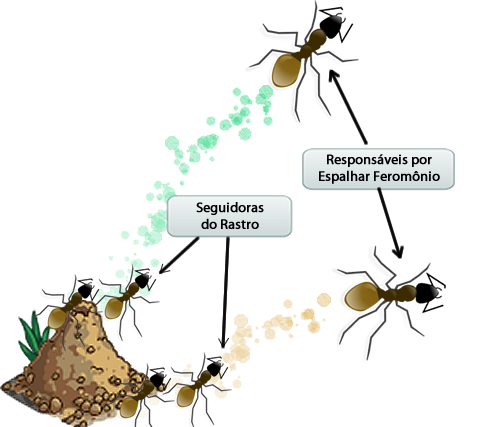
\includegraphics[width=12cm]{pictures/ants.png}
 \caption{Fenômeno Biológico de Distribuição de Feromônio.}
  \label{fig:ants}
 \end{figure}

Para a composição destes rastros é utilizada uma heurística inspirada em fenômenos biológicos, mais especificamete no comportamento de formigas quando buscam alimento.
O princípio deste comportamento, de forma simplificada,  é que uma formiga libera seu rastro através de um caminho no momento em que começa sua viagem em busca de alimento. Este rastro é composto por feromônios que exalam um odor específico para marcar o caminho percorrido. Um ponto importante a se ressaltar é que este rastro se evapora com o passar do tempo, isto, por fim, resulta em um gradiente que decresce de acordo com o tempo. Consequentemente, este caminho possuirá duas extremidades, uma extremidade com baixo valor de feromônio (início do caminho) e uma extremidade com altíssima concentração de feromônio (posição atual da formiga). Este rastro possibilita que a formiga (detentora do rastro) possa ser alcançada por qualquer outro indivíduo (outras formigas) que possua capacidades de interpretar o odor do feromônio.

A figura \ref{fig:ants} demonstra o fenômeno descrito.



Inspirado no comportamento anteriormente descrito, torna-se possível criar uma adaptação do mesmo para implementação no uso de redes de sensores sem fio em conjunto com veículos aéreos não tripulados. Para isso, basta que se considere um \vant como uma formiga capaz de produzir um rastro feromônio. Este rastro resultará em uma espécie de \emph{backbone} de feromônios que otimizará a entrega de mensagens destinadas ao \vant. A estratégia utilizada para que este comportamento fosse mapeado para uma rede de sensores pode ser dividida em duas responsabilidades:

\subsection{Entrega de Feromônios pelos \vants}
Cada \vant sobrevoando a área de interesse exala seus feromônios digitais periodicamente durante seu vôo. Utilizando recursos de comunicação sem fio, o \vant simplemeste enviará pacotes \emph{beacon} periodicamente em \emph{broadcast}. Este comportamente garante que os pacotes são enviados a todo momento para todos os nós sensores que se encontram no alcance do raio de comunicação do \vant. Um ponto interessante a se ressaltar é o \vant deve enviar, em cada pacote, um atributo que indique o "sabor" de feromônio que este \vant possui. Isto garante que no caso de vários \vants sobrevoando a área de interesse os rastros não se sobreponham, de modo que em um mesmo local possam ser armazenador rastros distintos.

A figura \ref{fig:broadcast} demonstra o item apresentado.

 \begin{figure}[h!]
 \centering
 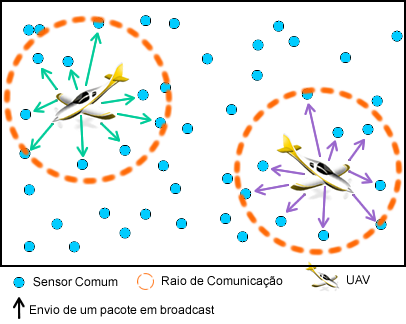
\includegraphics[width=10cm]{pictures/broadcast.png}
 \caption{Envio de um pacote em broadcast. Cada cor nas setas representa um sabor de feromônio.}
  \label{fig:broadcast}
 \end{figure}

\subsection{Armazenamento por parte dos Nós Sensores}
Os nós sensores espalhados pela área são responsáveis por armazenar os feromônios distribuídos pelos \vants, de modo a reproduzirem os rastros. Cada nó, ao receber um pacote enviado por um \vant deverá armazenar o sabor de feromônio recebido. Esta ação, quando observada em nível macro (todas as micro-ações produzidas por cada nó), resultará em um comportamento global, construindo rastros de feromônios digitais que representam os caminho percorridos por cada \vant dentro da área de interesse. 

 \begin{figure}[h!]
 \centering
 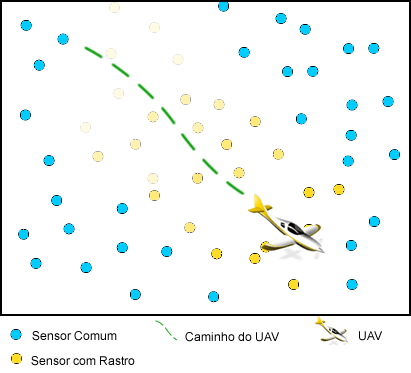
\includegraphics[width=10cm]{pictures/flat_pheromone.png}
 \caption{Pheromônios esmaecendo em função do tempo.}
  \label{fig:flat}
 \end{figure}

Além de armazenar o valor de feromônio recebido, o nó sensor deve agendar uma tarefa interna para reduzir (evaporar) seu valor de feromônio de acordo com o tempo. Um exemplo de tarefa é reduzir em vários intervalos de tempo o valor de feromônio armazenado a uma taxa de 10\%, de modo a simular a evaporação do feromônio. 
Esta evaporação garante que o rastro mantenha-se em maior concentração de feromônio na extremidade onde se encontra o \vant, e, em menor concentração na extremidade onde o rastro se originou.



Cada nó sensor armazenando os valores de feromônios representa o caminho por onde o \vant sobrevoou. Contudo, este rastro ainda pode conter certas ambiguidades. Observando-se o fato que diversos nós sensores recebem o mesmo valor de feromônio, verifica-se que em uma mesma região contida no raio de alcance do \vant (considerando-se que a propagação do sinal ocorre em diversas direções) existem diversos nós sensores representando a mesma quantidade de feromônio, como demonstrado na figura \ref{fig:flat}. Ainda que os valores evaporem com o tempo, seguindo esta tendência, os nós sensores evaporarão com a mesma proporção, resultando em um rastro que somente encaminhará as mensagens a uma região (do mesmo tamanho do raio de propagação do \vant), não a um ponto específico na rede. Neste caso, encaminhar a mensagem a uma região pode não ser o ideal, visto que a mensagem não encontraria um sentido correto para ser encaminhada.



Para sobrepor esse problema, pode-se adicionar uma restrição ao se armazenar um valor de feromônio em um dado nó sensor. Neste caso, em específico, utiliza-se a informação de intensidade com que o pacote foi recebido (RSSI) pelo nó sensor. A informação recebida garante que se armazene valores de feromônio proporcionais à distância entre os nós sensores e o emissor dos pacotes. Este armazenamento promoverá, em nível macro, um rastro em formato de gradiente, que será resultante da variação dos valores de feromônio em relação ao tempo em que o nó sensor recebeu o pacote e à distância entre o nó sensor e o \vant emissor do pacote. Este gradiente é demonstrado na figura \ref{fig:gradient}.

 \begin{figure}[h!]
 \centering
 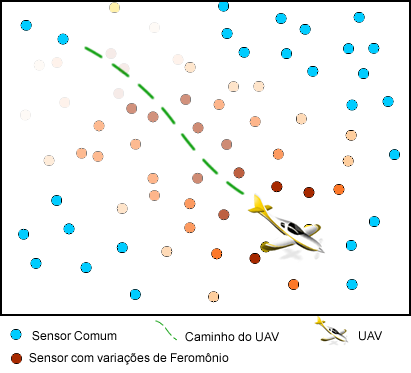
\includegraphics[width=10cm]{pictures/gradient.png}
 \caption{Pheromônios esmaecendo em função do tempo e da distância relativa ao \vant. Os toms de vermelho variam de acordo com a distância do nó sensor em relação ao \vant, bem como varia a transparência do nó em relação ao tempo.}
  \label{fig:gradient}
 \end{figure}


\subsection{Propagação de Eventos}
Uma vez detectado um evento de interesse, espera-se que o sistema seja capaz de reportá-lo ao \vant mais adequado para tratar o fenômeno com maior granularidade. Para o alcance de tal objetivo é utilizado um algoritmo de propagação de eventos. Este algoritmo integra os dois algoritmos anteriores, de modo que se torne possível a entrega dos eventos aos \vants.

O primeiro passo para o funcionamento deste algoritmo é a definição de alarme. Neste contexto um alarme é considerado como uma estrutura de dados responsável por carregar informações acerca do evento ocorrido. A estrutura de um alarme é formada por:

\begin{description}
	\item[\emph{Position}:]  Representa a posição em que o evento foi detectado.
	\item[\emph{TimeStamp}:] Informa o momento em que o alarme foi disparado.
	\item[\emph{PheromoneAmmount}:] Indica a quantidade atual de feromônio presente no alarme. Esta quantidade de feromônio é o principal atributo presente nesta estrutura de dados, pois será atualizada cada vez que o alarme for repassado.
	\item[\emph{Flavor}:] Fornece o "sabor" de feromônio mais propício a tratar este evento. Por exemplo, no caso da detecção de um evento sonoro, o sabor do alarme seria "\emph{noise}", de modo que este alarme somente deve ser repassado para nós sensores que possuam feromônios do sabor \emph{noise}.
\end{description}

O funcionamento básico desta propagação de eventos baseia-se em repassar o alarme do ponto inicial (ponto de detecção do evento) ao ponto final (posição do \vant). Visto que neste ponto já existem diversos gradientes formados pelos rastros dos \vants, a tarefa do nó sensor detector do evento resume-se em determinar o "sabor"  que mais se adequa ao evento em questão e encaminhar o alarme, de modo que o mesmo alcance seu destino (\vant mais apropriado).

Para a propagação do alarme criado, o nó sensor deve encaminhá-lo somento a outros nós sensores que estejam dentro do mesmo rastro de feromônio. Uma observação importante neste método é que o alarme só deve ser encaminhado para nós sensores que possuam concentração de feromônio superior ao do nó sensor criador do alarme. Para que essa premissa seja garantida,  torna-se imprescindível que a estrutura de Alarme carregue a informação da quantidade de feromônio presente no alarme. Seguindo-se esta idéia, o nó sensor detector deve encaminhar seu alarme em mensagens do tipo \emph{broadcast}, de modo que seus vizinhos recebem a informação de alarme. 

Uma vez que um vizinho do nó sensor propagador receber o pacote contendo o alarme, deverá analisar o alarme recebido e decidir se encaminha a mensagem ou não.  Se a quantidade de feromônio armazenada no nó sensor receptor for menor que a quantidade do alarme, o nó receptor simplesmente deve descartar o alarme. Contudo, se a quantidade armazenada no nó receptor for superior à quantidade de feromônio recebida, o nó receptor deve atualizar atualizar o valor de feromônio do alarme com seu próprio valor e repassar a mensagem também em formato de \emph{broadcast}. 

A execução das pequenas e locais ações anteriores acarretará em um comportamento global em toda a rede de sensores. Estas interações entre os nós sensores promoverão a entrega da mensagem contendo o alarme ao \vant que estiver sobrevoando a área de interesse no momento em que se detectou o evento.

O algoritmo básico, em psedocódigo, para este fenômeno pode ser visualizado abaixo: \\


\begin{algorithm}[H]
%	\SetAlgoLined
	
	\SetKwFunction{minhaQuantidadeDeFeromonio}{minhaQuantidadeDeFeromonio}
	\SetKwFunction{encaminharAlarme}{encaminharAlarme}

	\Entrada{Objeto Alarme}

	\Se{ alarme.quantidadeDeFeromonio < \minhaQuantidadeDeFeromonio() }{
			alarme.quantidadeDeFeromonio = \minhaQuantidadeDeFeromonio()\;
			\encaminharAlarme(alarme);
		}
	
\caption{Algoritmo para a propagação de eventos.}
\end{algorithm}


\begin{figure}[h!]
\centering
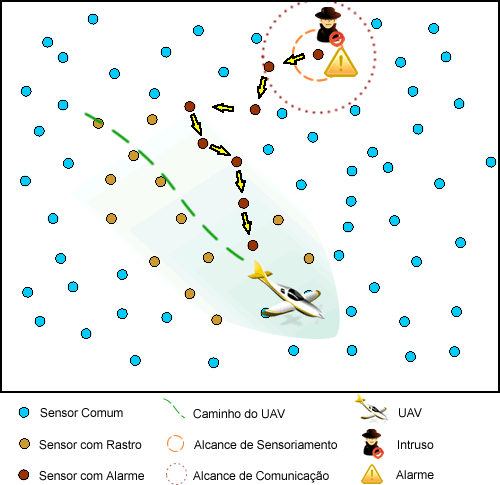
\includegraphics[width=12cm]{pictures/application.png}
\caption{Propagação de um evento de interesse.}
 \label{fig:app}
\end{figure}

Uma particularidade interessante deste algoritmo é que podem exister regiões na área de interesse em que ainda não se existe a presença de rastros de feromônio. Contudo, esta questão apresenta-se discutível, pois poderia-se considerar que o sistema só entraria em funcionamento no momento em que toda área já estivesse coberta pelo \vant. Entretanto, esta premissa não pode ser garantida em todos os casos. Para que este problema seja contornado, pode ser proposta uma variação deste algoritmo em que quando um nó sensor detectar um evento e o mesmo não possuir rastro de feromônio, este nó deverá encaminhar a mensagem para um de seus vizinhos, na esperança de que este visinho possua rastros. Existem algumas medidas para que se escolha o vizinho mais adequado para receber a mensagem de alarme. Contudo, devido a extensibilidade da explicação, não serão abordadas neste trabalho. Porém, vale ressaltar que esta particularidade ocorre em poucos casos e será abordada novamente no capítulo de resultados.

 A figura \ref{fig:app} demonstra um exemplo do funcionamento básico da propagação de eventos.
 



%\subsection{Reforço da Conectividade da Rede}
%Esta seção aborda um último algoritmo deste trabalho. É válido salientar que este esta última técnica não influencia diretamente os resultados dos algoritmos apresentados anteriormente. Entretanto, as melhorias propostas nas seções anteriores propiciam o cenário para a implementação deste último algoritmo.

%O algoritmo de Reforço de Conectividade da Rede utiliza os \vants que sobrevoam a área de interesse como nós sensores móveis, de modo que os \vants possam complementar a conectividade da rede em caso de falhas em nós sensores. Basicamente, falhas em nós sensores pode, ser consideradas como indisponibilidade de energia, falha em sensores, falha na interface de comunicação, etc.

%Uma falha pode ser detectada pelo próprio nó, ou por seus vizinhos. Um exemplo de falha detectada pelo próprio nó é o mal funcionamento de um sensor, ou níveis muito baixos de energia. Falhas detectadas por vizinhos podem ser falência de um nó sensor ou ausência de interface de comunicação (não responde às mensagens de seus vizinhos), etc. A principal característica a se observar neste caso é que este problema pode ser mapeado em termos dos problemas anteriores; uma falha em um nó sensor pode ser considerada como um evento de interesse, e os rastros de feromônios podem ser utilizados para se carregar a mensagem de falha até o \vant mais próximo.

%Ao receber uma mensagem de falha de um nó sensor, o \vant deve se preocupar em cobrir a conectividade da rede naquela região, atuando como um nó sensor da rede. Contudo, o \vant ainda possui suas responsabilidades em relação ao sistema de monitoramento de eventos. Para que se torne possível que o \vant realize todas as suas tarefas, a estratégia empregada é que o \vant apenas visite a área de falha em um determinado intervalo de tempo, e depois prossiga com seu itinerário.

%Quando um \vant recebe mais de um alarme de falha de sensor, torna-se necessário que exista um escalonamento para que o \vant visite todas as regiões de falha. No desenvolvimento deste escalonamento, optou-se por uma implementação baseada em políticas. Neste caso, foi determinado um protocolo\footnote{Também pode ser considerado como uma Interface nos conceitos de Orientação a Objetos.} para a implementação de diferentes políticas. Isto permite que se desenvolva diferentes estratégias para o escalonamento das visitas às regiões de baixa cobertura da rede. Dentre estas políticas, podem ser destacadas:

%\begin{description}
%	\item[Agrupamento por Proximidade:] política para que o itinerário de visitas do \vant baseie-se em visitar sempre os nós mais próximos, de modo que a próxima região de visita seja a de menor distância do ponto atual.
%	\item[Agrupamento Crítico:] é uma política em que se preocupa, principalmente, no agrupamento dos nós de acordo com a criticidade da região de falha. Nesta estratégia, a primeira região a ser visitada é a que possui mais avarias.
%	\item[Agrupamento por Proximidade do \vant:] é uma especialização da primeira política. Todavia, mais complexa de se implementar, visto a necessidade de atualização da rota de acordo com a movimentação do \vant.
%\end{description}

%Uma característica interessante desta abordagem é a possibilidade de se alternar as políticas nos momentos mais adequados. Um \vant pode trabalhar com uma política A e ser reprogramado, ainda que em operação, para utilizar uma política B. Ainda mais, diversos \vants, no mesmo cenário, podem empregar diferentes políticas para o reforço de conectividade da rede. Ampliando, assim, o dinamismo do algoritmo abordado.

%O protocolo para implementação desta políticas, apesar de dinâmico, apresenta-se simples, o desenvolvedor deve apenas oferecer um procedimento que compare duas regiões de falha.

%Os blocos de código a seguir ilustram a implementação de uma política utilizada no trabalho.

%\begin{lstlisting}[caption=Procolo (Interface) para implementação de Políticas de Agrupamento.]
%package br.ufla.dcc.ucr.node.data;
%public interface CoverageInfoComparator {
%	int compare(CoverageInformation me, CoverageInformation other);
%}
%\end{lstlisting}


%\begin{lstlisting}[caption=Implementação de Agrupamento Crítico.]
%package br.ufla.dcc.ucr.node.data;
%/**
%*  Neste caso, coverage indica o grau de cobertura do no. Isto significa o quao danificado um no se encontra.
%*/
%public class SortByCoverage implements CoverageInfoComparator {
%	@Override
%	public int compare(CoverageInformation me, CoverageInformation other) {
%		if (me.getCoverage() == other.getCoverage())
%			return 0;
%		if(me.getCoverage() < other.getCoverage()){
%			return 1;
%		}else{
%			return -1;
%		}
%	}
%}
%\end{lstlisting}


%\begin{lstlisting}[caption=Escolha da Política]
%package br.ufla.dcc.ucr.node.data;
%...
%public class CoverageInformation implements Comparable<CoverageInformation> {
%	//Escolha da politica de Agrupamento Critico. Basta mudar esta linha para trocar %a politica.
%	private CoverageInfoComparator compareStrategy = new SortByCoverage();
%	...
%	@Override
%	public int compareTo(CoverageInformation other) {
%%
%	}
%	...
%}
%\end{lstlisting}

%Para este trabalho, foram desenvolvidas as políticas de Agrupamento por Proximidade e de Agrupamento Crítico. Contudo, o modelo proposto permite que diversas extensões sejam feitas ao algoritmo.

O próximo capítulo demonstra os resultados dos experimentos realizados com os algoritmos apresentados neste capítulo.

\newpage\section{Resultados e Discussão}
\label{chap:Resultados}

Este capítulo apresenta discussões acerca dos resultados obtidos nos experimentos do algoritmo desenvolvido neste trabalho, abordando os resultados das simulações envolvendo o processo de construção dos rastros de feromônio e detecção e propagação dos eventos. 
%A segunda demonstra os resultados das simulações ao se adicionar o comportamento de reforço da conectividade da rede, onde são apresentados os resultados da combinação das estratégias, bem como os resultados da utilização independe do último algoritmo.

\subsection{Construção dos Rastros de Feromônio e Propagação de Eventos}
Os experimentos realizados para avaliar o desempenho da técnica desenvolvida no trabalho foram baseados na comparação desta técnica com uma abordagem tradicional: o envio de mensagens por \emph{flooding}. No caso da propagação de mensagens por \emph{flooding}, quando um evento é detectado, o nó sensor detector envia o alarme em \emph{broadcast} e todos os seus vizinhos repetem este alarme (também em \emph{broadcast}), de modo que todos os nós do sistema repitam o alarme, até que, em algum momento, a mensagem chegue ao \vant de destino.

As métricas avaliadas nesta comparação foram:

\begin{description}
\item[a) Número total de Mensagens: ] representa o número total de mensagens utilizadas para enviar um alarme até seu destinatário.
\item[b) Número de Saltos:] o número de saltos realizados por um alarme desde seu emissor até seu receptor. Este valor representa a quantidade de nós intermediários entre o nó emissor e o \vant receptor do alarme.
\end{description}

\subsection{Configurações da Simulação}
Foram realizadas 200 simulações (100 simulações em cada técnica). Os experimentos foram realizados com o intuito de avaliar o comportamento da rede de forma isolada no acontecimento de um evento de interesse. Portanto, optou-se por simular um cenário contendo apenas um \vant e com a ocorrência de apenas um evento de interesse, de modo que se consiga visualizar o comportamento específico do envio de mensagens através do \emph{backbone} sem a interferência de muitos eventos. O intervalo de tempo em que as métricas são analisadas é o tempo necessário para a ocorrência de um evento em adição ao tempo gasto para que a mensagem alcance seu destino.

A escolha dos parâmetros de configuração da simulação, em relação às capacidades dos \vants, foi determinado baseando-se no uso de Mini e Micro-\vants. Baseando-se nas informações em \cite{uas_2009,Storvold2009}, optou-se por uma altitude de 250 metros. Em relação aos nós sensores terrestres, foram simuladas as funcionalidades de rádios semelhantes àqueles que seguem o padrão IEEE 802.15.4.

Neste cenário, quando um \vant não está respondendo a um alarme deve realizar sua rota de forma aleatória, de modo a construir seu rastro de feromônio. São distribuídos 140 nós sensores terrestres (com raio de comunicação de 300m) seguindo a distribuição de Poisson em uma área de 2Km x 2km, obtendo-se aproximadamente 100\% de probabilidade de que os nós formem um grafo conexo \cite{Bettstetter2002}.

A Tabela \ref{tbl:setup} resume os parâmetros utilizados para as simulações.

\begin{table}[h!]
\centering
	\begin{tabular}{| l | l |}
		\hline
		Parâmetro & Valor \\
		\hline
		Cenário (Área)  & 2 Km x 2 Km\\
		Raio de Comunicação do \vant & 400m\\
		Altitude de Vôo & 250m  \\
		Número de nós sensores estáticos & 140  \\
		Raio de comunicação dos nós sensores & 300m \\
		\hline
	\end{tabular}

	\caption{Parâmetros para simulação da Construção dos Rastros de Feromônio e Propagação de Eventos.}
	\label{tbl:setup}
\end{table}

A Tabela \ref{tbl:setup_network} apresenta as configurações da rede utilizada nos experimentos.
\begin{table}[h!]
\centering
	\begin{tabular}{| p{10cm} | l |}
		\hline
		\multicolumn{2}{|c|}{\textbf{Configuração}} \\
		\hline
		Composição  & Heterogênea\\
		\hline
		Organização & Plana\\
		\hline
		Mobilidade & Móvel  \\
		\hline
		Densidade & Balanceada  \\
		\hline
		Distribuição & Irregular \\
		\hline
		
		\hline
		\multicolumn{2}{|c|}{\textbf{Sensoriamento}} \\
		\hline
		Coleta  & Periódica\\
		\hline
		
		
		\hline
		\multicolumn{2}{|c|}{\textbf{Processamento}} \\
		\hline
		Cooperação  & Localizada\\
		\hline
		
	\end{tabular}

	\caption{Parâmetros da Rede de Sensores utilizada para os experimentos.}
	\label{tbl:setup_network}
\end{table}


\subsubsection{Resultados}

 A Figura \ref{fig:hops} demonstra os resultados da simulação em relação ao número de saltos ocorridos até que o \vant recebesse o alarme. O eixo x representa o número da simulação e o eixo y representa o número de saltos necessário para que o alarme alcançasse o destino. Pode-se notar uma proximidade nestes resultados em relação aos valores, isto deve-se ao fato de que esta métrica avalia o caminho percorrido pelo alarme em um mesmo cenário para ambas as simulações. É importante verificar que no algoritmo baseado em feromônios, a mensagem percorre uma única faixa (caminho) até alcançar seu receptor. Em contrapartida, na estratégia baseada em \emph{flooding}, são percorridos todos os possíveis caminhos contidos no grafo formado pelos nós sensores. Isto implica que em um determinado momento, dentre todos os caminhos, um deles encontrará o \vant. Neste caso, o número de saltos com valores próximos é justificado pelo fato de que um dos caminhos encontrados na estratégia de \emph{flooding} (exatamente o caminho que foi contabilizado no experimento) é um caminho muito parecido com o utilizado pelo algoritmo de feromônio. A Figura \ref{fig:hops_mean} apresenta a média dos resultados para este experimento. Adicionalmente, a Figura \ref{fig:hops_hist} demonstra o histograma dos dados em relação a essa métrica.


 \begin{figure}[h!]
 \centering
 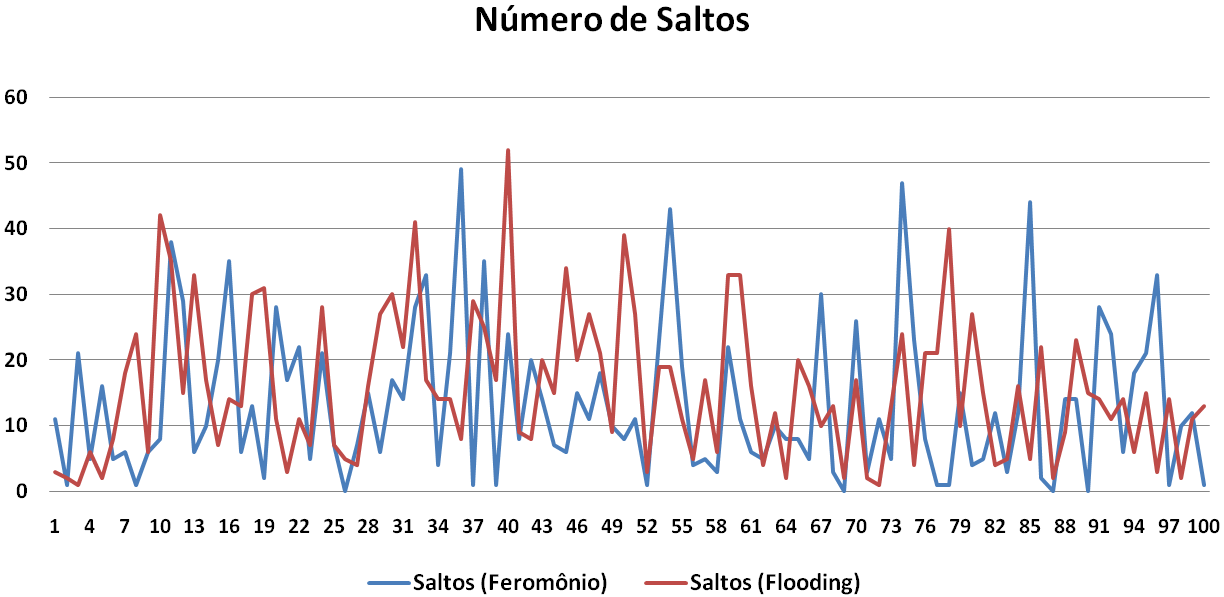
\includegraphics[width=13cm]{results/hops.png}
 \caption{Resultados em relação ao número de saltos.}
  \label{fig:hops}
 \end{figure}


 \begin{figure}[h!]
 \centering
 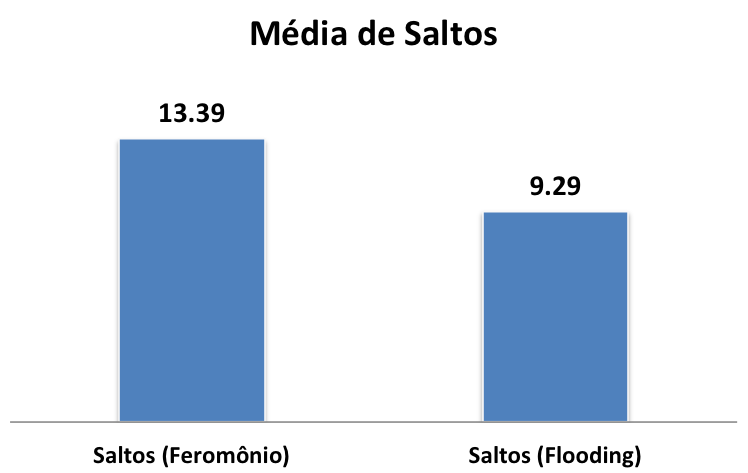
\includegraphics{results/hops_mean.png}
 \caption{Média do Número de Salto.}
  \label{fig:hops_mean}
 \end{figure}

\begin{figure}[h!]
 \centering
 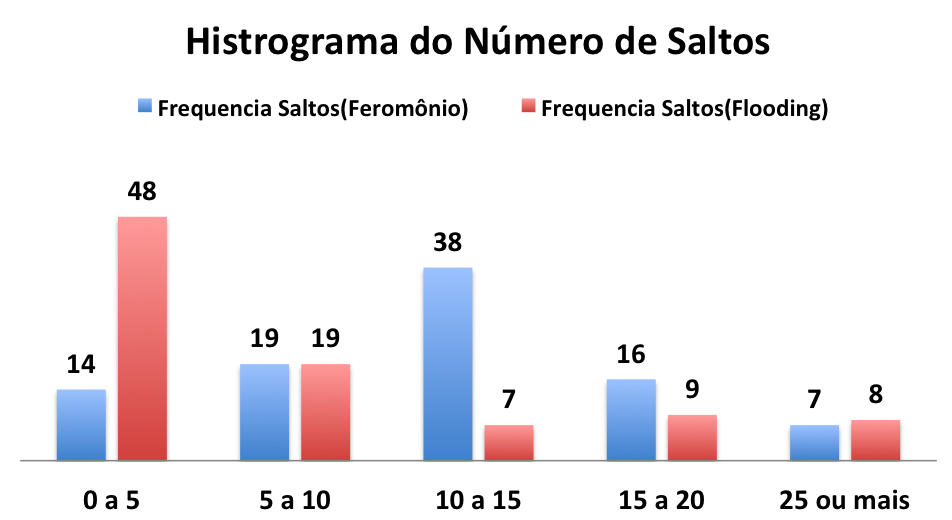
\includegraphics[width=13cm]{results/hops_hist.png}
 \caption{Histograma do Número de Saltos.}
  \label{fig:hops_hist}
 \end{figure}

Os resultados anteriores não justificam a utilização do algoritmo de feromônios. Contudo, ao se analisar os resultados em relação ao número de mensagens enviadas, é possível verificar a eficiência deste algoritmo em relação ao método tradicional de \emph{flooding}. As figuras \ref{fig:messages}, \ref{fig:messages_mean} e \ref{fig:messages_hist}, respectivamente, exibem os resultados obtidos em cada simulação, a média e o histograma do número de mensagens enviadas pelo sistema durante a entrega de um alarme. Nota-se uma relação na ordem de aproximadamente 8 vezes nos resultados para o número de mensagens. Este resultado complementa os dados apresentados anteriormente, mostrando a real diferença entre as duas técnicas. A diferença pode ser vista pelo fato de que, mesmo realizando valores de saltos muito próximos, os algoritmos diferenciam-se na quantidade utilizada de mensagens para a entrega de um alarme. O uso do rastro de feromônio garante que somente um caminho será tomado para a busca do \vant, ao contrário da abordagem tradicional, em que todos os possíveis caminhos são verificados.

 \begin{figure}[h!]
 \centering
 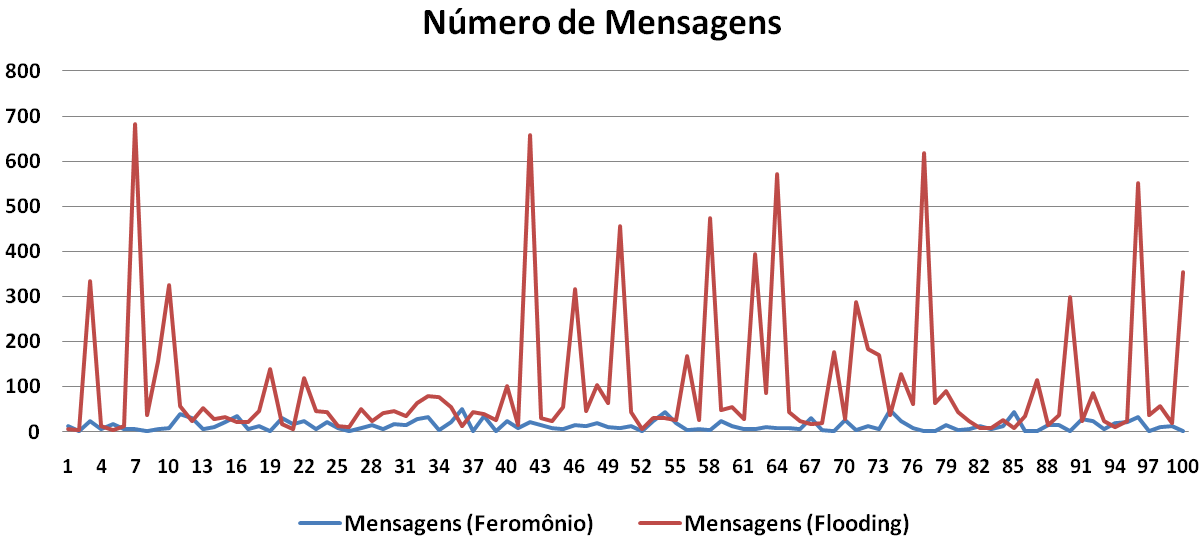
\includegraphics[width=13cm]{results/messages.png}
 \caption{Resultados em relação ao número de mensagens enviadas.}
  \label{fig:messages}
 \end{figure}

 \begin{figure}[h!]
 \centering
 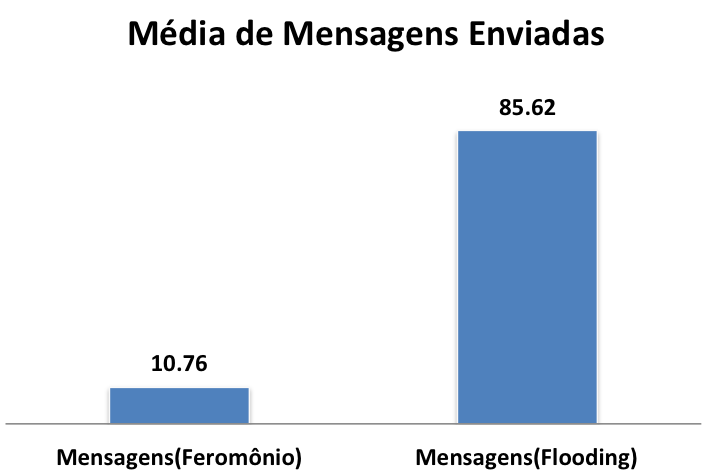
\includegraphics{results/messages_mean.png}
 \caption{Média do Número de Mensagens.}
  \label{fig:messages_mean}
 \end{figure}

\begin{figure}[h!]
 \centering
 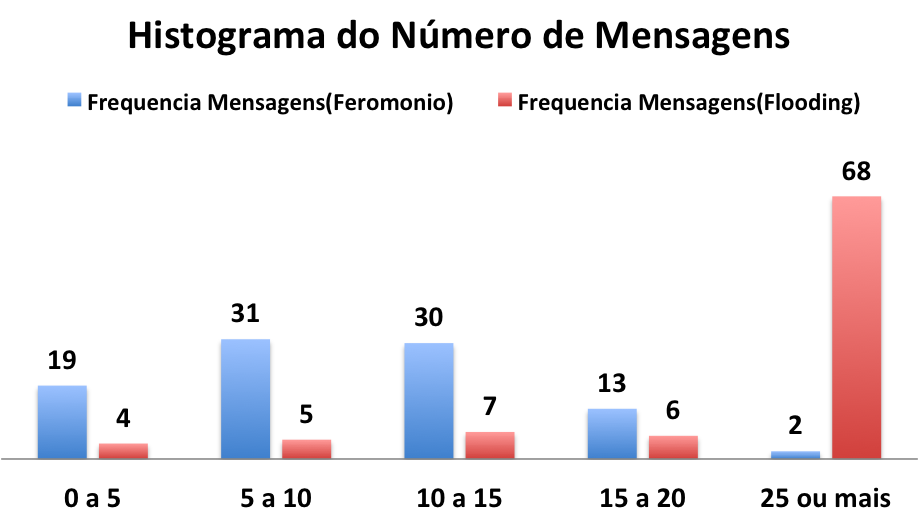
\includegraphics[width=13cm]{results/hist_messages.png}
 \caption{Histograma do Número de Mensagens.}
  \label{fig:messages_hist}
 \end{figure}

Os resultados demonstram a possibilidade de se reduzir o número de mensagens trafegadas em uma rede de sensores sem fio no que se refere a detecção e propagação de eventos em uma área de interesse. 

Os resultados comprovam a eficiência do uso do algoritmo utilizando rastros de feromônio para a entrega de alarmes na ocorrência de um evento de interesse. O próximo capítulo discute as considerações finais em relação aos resultados do trabalho desenvolvido.

\newpage\section{Conclusões}

Esta parte ainda não foi desenvolvida pois nem todos os resultados foram obtidos.
Em breve esta parte estará terminada.

\newpage

\bibliography{bib_tcc}
%==============================================================================
% Incluindo bibliografia
%\bibliographystyle{plain}             % estilo para labels em numeros
%\bibliographystyle{alpha}             % estilo para labels em iniciais
\bibliographystyle{abnt-alf}           % estilo para referências usando ABNT, 
                                       % precisa instalar o abntex para usar!!!
%\bibliographystyle{apalike}



\end{document}
